\chapter{The GOTO Telescope Control System}
\label{chap:gtecs}
\chaptoc{}

% ########################################

\newpage
\section{Introduction}
\label{sec:gtecs_intro}
\begin{colsection}

% ~~~~~~~~~~~~~~~~~~~~

\begin{colsection}

This chapter describes \rtxt{<blah> <blah>}.
I did most of the work with the help of Vik and Stu and so on.
It's based on my SPIE paper, plus some GOTO talks.

\end{colsection}

% ~~~~~~~~~~~~~~~~~~~~

\subsection{Requirements of the control system}
\label{sec:control_requirements}
\begin{colsection}

My first task as part of the GOTO collaboration, in the summer before I started in Sheffield, was to decide on what control system software to use for the telescope. There were several requirements to consider.

Firstly the chosen system had to allow for remote and, most importantly, robotic operation of GOTO.\@ There are many telescope software packages available, but the majority are designed for a human observer to operate. GOTO however was to be a fully autonomous telescope, which meant operating nightly with no human intervention. This meant the control system had to contain routines for observing targets and standard tasks like taking calibration frames. On top of that it was desirable for the system to be able to monitor itself to detect and fix any errors as much as possible without the need for human intervention. Finally it had to be able to monitor and react to external conditions, for example closing the dome if rain was detected.

Secondly the system had to include an observation scheduler, which could decide what the telescope should observe during the night. A basic scheduler might be run in the evening to create a night plan, as observers typically do when operating a telescope. However that alone would not fit the expected operations required from GOTO:\@ normally carrying out an all-sky survey but with a robust interrupt protocol for gravitational wave follow-up. The system therefore had to be able to recalculate what to observe on-the-fly, and be able to immediately react to transient \gls{too} events.

Furthermore, although the project was still at an early stage the idea of linking together multiple telescopes into a global network was also considered, and the chosen control system implementation would ideally be expandable to facilitate this in the future (or at least not hinder the possibility).

There were also several physical considerations when it came to choosing between software systems. The telescope hardware had already been decided on: an Astrohaven clamshell dome\footnote{Astro Haven Enterprises, CA, USA;\@ (\url{www.astrohaven.com})}, a custom mount with a \gls{sitech} servo controller\footnote{Sidereal Technology, OR, USA;\@ (\url{www.siderealtechnology.com})} and multiple unit telescopes all using \gls{fli} cameras, focusers and filter wheels\footnote{Fingerlake Instruments, NY, USA;\@ (\url{www.flicamera.com})}. Any control system would need to communicate with all of them, so any systems with existing drivers or packages used by established projects would be desirable.

Two particular hardware-related challenges faced the control system project. The first was that the SiTech controller software, \software{SiTechEXE}, only ran on Microsoft Windows. The software did have an accessible \gls{api} through the \software{ASCOM} standard\footnote{\url{www.ascom-standards.org}} but that still required some form of the mount control system to be running on Windows. As most scientific software in astronomy runs on Linux systems this lead to two options: either have just a small interface running on the Windows machine and the majority of the system on Linux, or have the entire system run on Windows.

The second challenge was to deal with the multiple-unit telescope design of \gls{goto}. A full array of eight \glspl{ut} would require eight cameras, focusers and filter wheels. These would all need to be run in parallel, most importantly there needed to be no delay between the exposures starting and finishing on each camera. The physical construction of the telescope also came into play. The \gls{fli} units all require a USB connection to the control computer. A single computer situated in the dome would therefore require 24 USB cables to run up the mount, not only a practical difficulty but also a layout that could lead to interference and data loss. The suggested solution was to have small computers attached to the mount boom arms to act as intermediate interfaces to the \gls{ut} hardware. The control system therefore needed to be able to run in a distributed manner across multiple computers, potentially even running different operating systems.

Finally, there were practical details to consider. \gls{goto} was designed as a relatively inexpensive project that could be built quickly and copied across multiple sites, therefore any costly software licenses would ideally be avoided. Experience and support requirements should also be considered, and reusing a system that members of the collaboration had experience with would provide benefits compared to a completely new and exotic system.

\end{colsection}

% ~~~~~~~~~~~~~~~~~~~~

\subsection{Different control system options}
\label{sec:control_options}
\begin{colsection}

Four possible options for the GOTO control systems were considered: the existing software packages \software{ACP Expert}, \software{Talon} and \software{RTS2} or a custom system based on the code written for the \gls{pt5m}. At the July 2015 GOTO meeting at Warwick University I gave a talk outlining the control system requirements and presenting the four options, and the decision taken was to adapt the \gls{pt5m} system for use by GOTO.\@ The three rejected systems are described below, while the \gls{pt5m} system is described in more detail in Section~\ref{sec:pt5m}.

\subsubsection{\software{ACP Expert}}
\software{ACP Expert}\footnote{\url{http://acp.dc3.com}} is a commercial observatory control software system by DC3-Dreams. It is used by some advanced amateur astronomers and a few scientific and university telescopes, such as the Open University's \gls{pirate} \citep{PIRATE}. As a complete Windows software package with a web interface it is marketed as being straightforward to use, in either remote or fully robotic modes. It uses the \software{ASCOM} standard library and DC3-Dreams also provide professional support and updates. This however came at a cost: \$2495 for the base software, plus an additional \$599 for Maxim DL camera control and \$650 per year for continued support. At the time \gls{goto} was anticipated to be deployed in a matter of months, so the quick and simple pre-existing commercial solution was tempting. However it was unsure if the \software{ACP} software would be able to cope with \gls{goto}'s unusual design, and its closed-source model would restrict our ability to make modifications.

\subsubsection{\software{Talon}}

The \software{Talon} observatory control system\footnote{\url{https://observatory.sourceforge.io}} is a Linux-based, open-source system created by \gls{omi}. It was included as an option primarily as at the time it was the control system of choice for the other observatories operated by Warwick University, such as SuperWASP \citep{SuperWASP}. \gls{omi} had built the SuperWASP mount and developed \software{Talon} alongside it, before later making it open source. However as a programme development has been limited to non-existent over the past decade, and Warwick were already looking at replacing it for their \gls{w1m} telescope and, ultimately, when upgrading SuperWASP.\@ Therefore adopting it for \gls{goto} would be unlikely and even counter-productive, as whatever was chosen for \gls{goto} was expected to (and ultimately did) influence and benefit the concurrent development of a new control system for \gls{w1m}.

\subsubsection{\software{RTS2}}

The \gls{rts2}\footnote{\url{https://rts2.org}} \citep{RTS2, RTS2b} is another free and open-source Linux software package. Unlike \software{Talon}, \software{RTS2} is under active development and is used by telescopes and observatories around the world \citep{BORAT, BOOTES-3, antarctic, ARTN}. There is a small but active community and multiple different drivers for the hardware \gls{goto} would use have been developed. The first version of RTS was written in \proglang{Python}, while the second version was rewritten in \proglang{C++} but with a \proglang{Python} interface available. \gls{rts2} was an attractive choice, however like the others it was unclear if it could be easily modified to meet the requirements for \gls{goto}'s multiple telescopes and Windows-controlled mount and no one in the collaboration had prior experience of using or implementing it.

\end{colsection}

% ~~~~~~~~~~~~~~~~~~~~

\subsection{The \textit{pt5m} control system}
\label{sec:pt5m}
\begin{colsection}

Built and operated by Sheffield and Durham Universities, \gls{pt5m} is a small \SI{0.5}{\metre} telescope located on La Palma on the roof of the \gls{wht} \citep{pt5m}. The telescope was originally developed as a \gls{slodar} system for atmospheric turbulence profiling \citep{SLODAR_LaPalma} and is one of several around the world operated by Durham, including one in Korea that had just been commissioned at the time I joined GOTO \citep{SLODAR_Korea}. In order to make the most of the telescope when not being used for \gls{slodar} observations a science camera was added to \gls{pt5m} and it was upgraded for robotic observations. Since it has successfully been used for automatic observations of transient events, as well as being used for undergraduate teaching at Sheffield and Durham. All the \gls{slodar} telescopes used a custom control system developed at Durham, and a similar system was used by the teaching telescopes of the Durham Department of Physics that I worked with during my undergraduate program. The \gls{pt5m} system has been modified for its extra roles which matched well to what we needed for \gls{goto}, and so it was chosen to be the base for the GOTO control system.

The \gls{pt5m} control system is written in \proglang{Python} and was built around multiple independent hardware daemon programs with a pilot program to control them. This basic framework was adopted for \gls{goto}, with some changes. The major obvious difference between \gls{pt5m} and \gls{goto} are the multiple unit telescopes, but the same system could be adapted through the creation of interface daemons on which allow communication to the unit telescopes over the network. In fact the nature of the daemon system made it very easy to expand to have daemons running on physically separate machines but still communicate over the network, including on both Linux and Windows computers. This also made it possible to run the scheduler and sentinel on the database machine, a key detail for the multiple-telescope system.

\begin{figure}[p]
\begin{center}
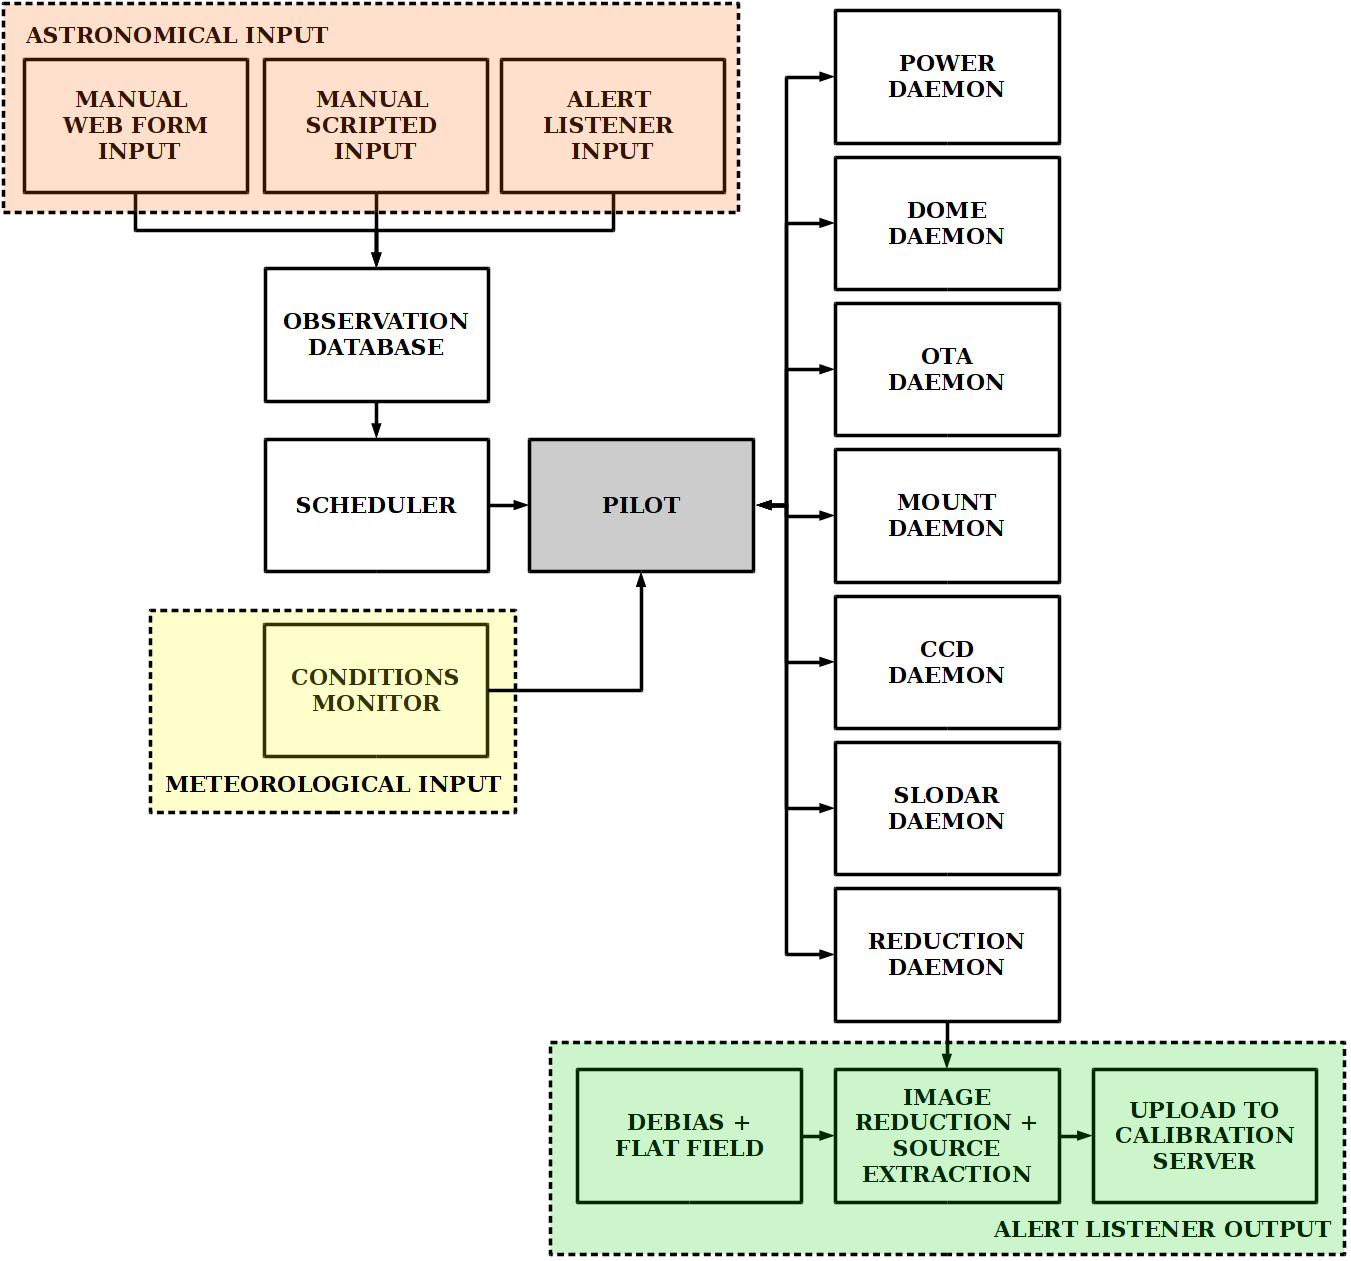
\includegraphics[width=\linewidth]{images/pt5m_software.png}
\end{center}
\caption[The pt5m control system architecture]{The \gls{pt5m} control system architecture, taken from~\cite{pt5m}. The hardware daemons are shown on the right, they communicate with the pilot which receives information from the observation scheduler and the conditions monitor. This basic framework was adapted for the GOTO control system, c.f. Figure~\ref{fig:flow}.}
\label{fig:pt5m_software}
\end{figure}

\end{colsection}

% ~~~~~~~~~~~~~~~~~~~~

\end{colsection}

% ########################################

\newpage
\section{Overview of G-TeCS}
\label{sec:gtecs}
\begin{colsection}

% ~~~~~~~~~~~~~~~~~~~~

\begin{colsection}

The \gls{gtecs} is the name given to the collection of programs and systems that have been developed to fulfil the requirements of the GOTO project. The \gls{pt5m} control system as described in the previous section formed the basis for \gls{gtecs}. Its structure of multiple independent daemons was developed into the core system architecture, shown in Fig.~\ref{fig:flow} below. This section gives an overview of the system and its implementation, and the following sections discuss in detail the two core branches of G-TeCS:\@ the base hardware control programmes (Section~\ref{sec:hardware_control}) and autonomous systems built on top of them (Section~\ref{sec:autonomous}).

\begin{figure}[h]
\begin{center}
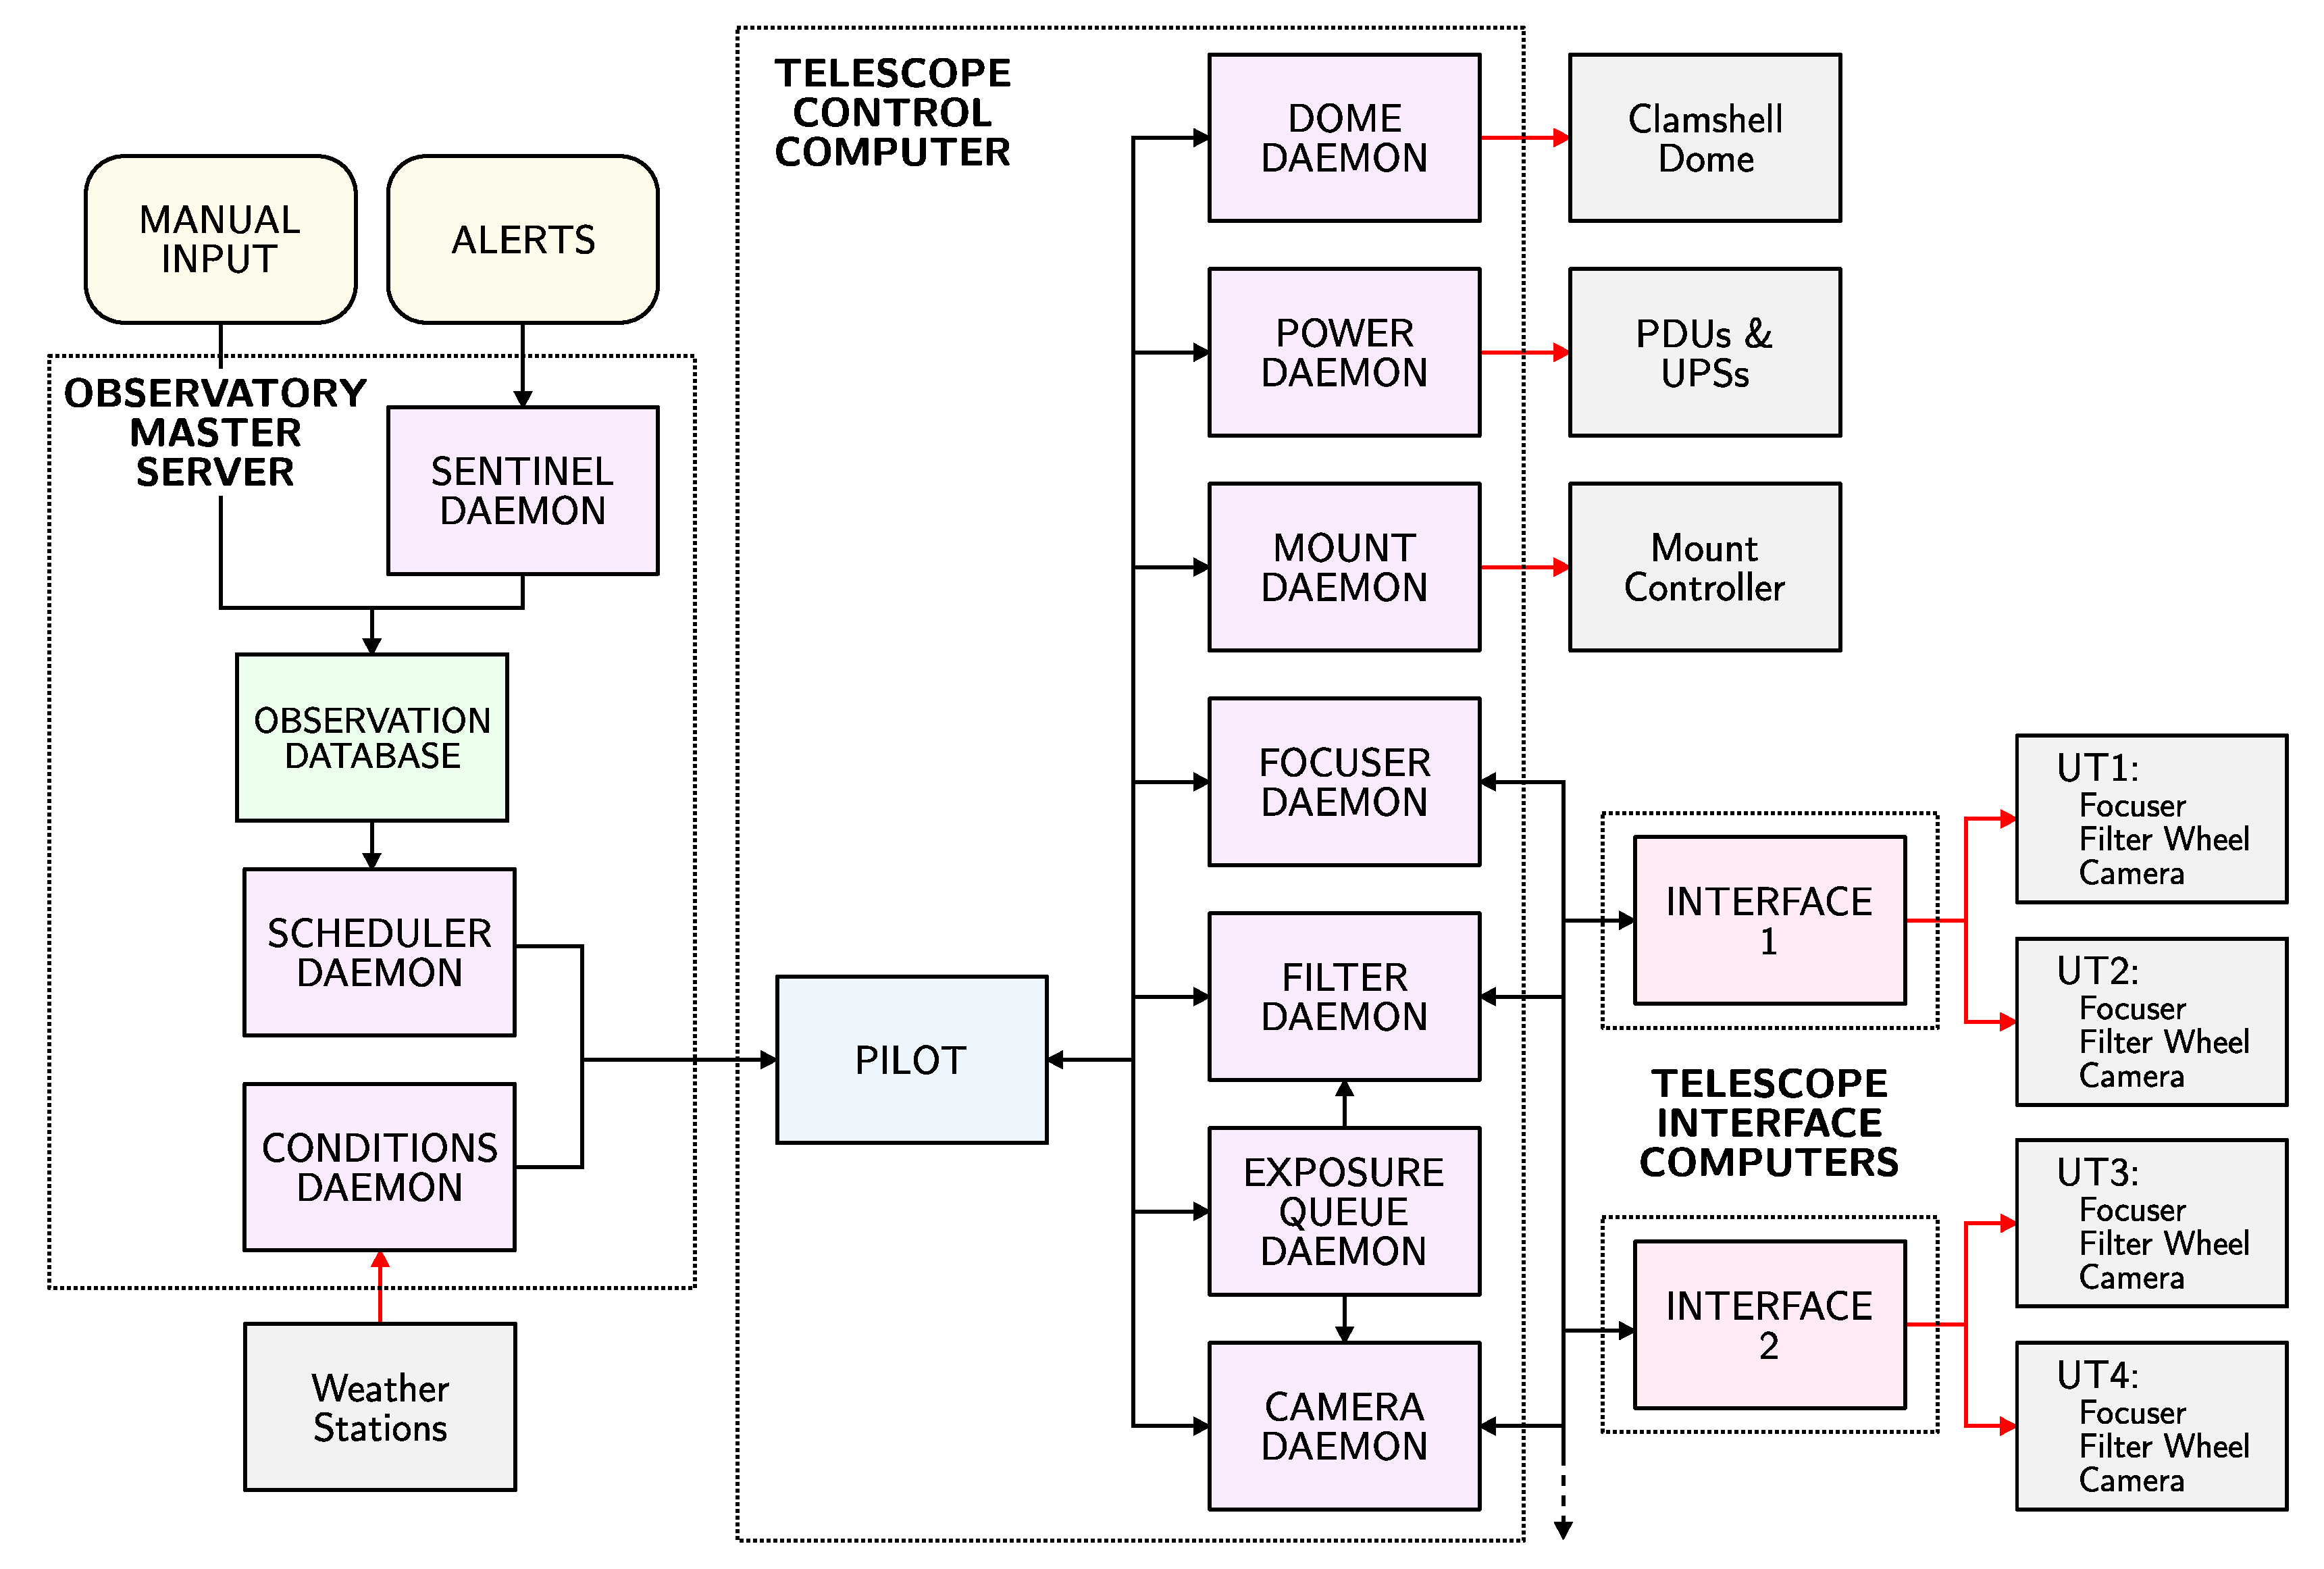
\includegraphics[width=\linewidth]{images/flow.pdf}
\end{center}
\caption[The G-TeCS system architecture]{The \gls{gtecs} system architecture as deployed on La Palma. The observation database as well as the sentinel, scheduler and conditions daemons shown to the left run on an observatory-wide master server, while the pilot and hardware daemons are located on the telescope control computer within the dome. Control for the unit telescope hardware (focuser, filter wheel and camera) is sent via an interface daemon for each pair of UTs, running on computers attached to the mount. Only the system for the prototype instrument (one mount with four unit telescopes) is shown.}
\label{fig:flow}
\end{figure}

\end{colsection}

% ~~~~~~~~~~~~~~~~~~~~

\subsection{Implementation}
\label{sec:implementation}
\begin{colsection}

The core \gls{gtecs} code is written as a \proglang{Python} package, \pkg{gtecs}. This includes all the daemons, scripts, associated modules and functions. One core component, the code and functions to interact with the observation database (see Section~\ref{sec:obsdb}), has been split off into a separate \proglang{Python} package ObsDB (\pkg{obsdb}), this was to allow other users to interact with the database without the need to install the entire \pkg{gtecs} package. In addition, the code for alert processing within the sentinel (see Section~\ref{sec:sentinel}) is in a separate module, GOTO-alert (\pkg{gotoalert}). This is because it originated as a separate code project developed by Alex Obradovic at Monash, that I then took over and integrated with the \gls{gtecs} sentinel.

G-TeCS and the associated packages are written almost entirely in \proglang{Python}, specifically \proglang{Python3}. \proglang{Python} is a versatile programming language that is increasingly common in astronomy, helped by the popular open-source Astropy Project \citep{astropy}. \proglang{Python} version 3.0 was released in 2008 and is infamously not backwards-compatible with \proglang{Python2}. The code for \gls{pt5m} was written in \proglang{Python2}, and therefore initially so was G-TeCS.\@ Over the subsequent years the code was re-written to be compatible with both \proglang{Python2} and \proglang{Python3}, which was possible due to the inbuilt \code{\_\_future\_\_} module in \proglang{Python2} and the \code{six} package. Finally the addition of new features added to \proglang{Python3}, such as the \pkg{asyncio} package (used heavily by the pilot) in version 3.5, and the imminent end-of-life of \proglang{Python2} in 2020 lead to the dropping of \proglang{Python2} support. This is in line with most other scientific \proglang{Python} packages including \pkg{astropy}, which is no longer developed for \proglang{Python2}. % chktex 21

The \pkg{gtecs} and associated packages have a variety of requirements. Some of the most critical external packages (not included in the \proglang{Python} standard library) are \pkg{numpy} for mathematical and scientific structures, \pkg{astropy} for astronomical functions, \pkg{sqlalchemy} for \proglang{SQL} database management (see Section~\ref{sec:obsdb}), \pkg{astroplan} for scheduling (see Section~\ref{sec:scheduler}), \pkg{voeventparse} for handling VOEvents (Section~\ref{sec:sentinel}) and \pkg{gototile} for sky map processing (Section~\ref{sec:gototile}).

\end{colsection}

% ~~~~~~~~~~~~~~~~~~~~

\subsection{Daemons}
\label{sec:daemons}
\begin{colsection}

The core elements of the control system are the daemons. A \emph{daemon} is a type of computer program that runs as a background process, continually cycling and awaiting any input from the user. This is in contrast to a \emph{script} which is run once (either by the system or a user), carries out a series of tasks in the foreground and then exits once it is completed. Common examples of daemons on a Unix-based system are \software{sshd}, which listens for and creates \gls{ssh} connections, and \software{cron}, which runs commands at predefined times. Incidentally both are used by G-TeCS:\@ \gls{ssh} to issue commands on remote machines and \software{cron} to start scripts like the pilot at a set time.

Daemons are the ideal form of software for hardware control. Once started each daemon runs continually as a background process, with a main control loop that repeats on a regular timescale (for the G-TeCS hardware daemons this is usually every \SI{0.1}{\second}). There are two primary tasks that are carried out within the loop by every daemon: monitoring the status of the hardware, and listening for and carrying out input commands. The former is typically not carried out every time the loop runs, because attempting to request and process the hardware status every \SI{0.1}{\second} would overwhelm the daemon and delay the loop. Instead the status checks are typically carried out every \SI{2}{\second}, or sooner if requested. By continually requesting the status of the hardware the daemon will detect very quickly if there are any problems, and should they be unable to reach their hardware they will enter an error state. However the daemons themselves will not attempt to self-diagnose and fix any problems that are detected, with the notable exception of the dome daemon (Section~\ref{sec:dome}). Instead that is the job of the hardware monitors (see Section~\ref{sec:monitors}), the daemons themselves will just report any problems to the pilot or user. The second reason for a control loop within the daemons is to listen for and carry out any commands issued to them. As these commands are dealt with within the loop it insures only one is carried out at once, the alternative of user input going directly to the hardware could cause problems with overlapping commands. These commands can be as simple as querying the cameras for how long left until an exposure finishes to opening the dome, taking and saving an image or calculating the current highest priority pointing to observe.

Within G-TeCS each category of hardware has a dedicated control daemon that acts as an interface to the hardware. For example, the mount daemon communicates with the SiTech mount controller, sending commands and reading the current status, while the camera daemon does the same for every camera attached to the telescope. Therefore there is not necessarily a one-to-one correspondence between daemons and pieces of hardware. Although typically grouped together as ``hardware daemons'' not every daemon within G-TeCS falls into that category: there is the scheduler daemon which is the interface to the observation database and the sentinel daemon which monitors alert channels. Although not connected to physical hardware like a dome or a camera, both operate in a similar way to the others.

Functionally each daemon is built around a \proglang{Python} class which contains hardware control functions and the main loop. When the daemon starts the loop is set running in its own thread, and when a control function is called it sets a flag within this loop to carry out the requested commands. The daemons are created using the \gls{pyro} module \pkg{Pyro4}\footnote{\url{https://pythonhosted.org/Pyro4/}}. Each daemon is run as a \gls{pyro} server, so any client script can then access its functions and methods across the network using the associated server ID.\@ This system allows complicated interactions across the network between daemons and scripts with very simple code, and was one of the major benefits of using the \gls{pt5m} system.

\end{colsection}

% ~~~~~~~~~~~~~~~~~~~~

\subsection{Scripts}
\label{sec:scripts}
\begin{colsection}

As well as the daemons, the \pkg{gtecs} package includes multiple \proglang{Python} scripts. Once installed these scripts can all be run from the command line by a human, or with utilities like \software{cron}.

In order to send commands to the daemons each has an associated control script that can be called by a user from a terminal, or by the pilot in robotic mode (see Sec~\ref{sec:pilot}). The commands follow a simple format which was inherited from \gls{pt5m}, first the short name of the daemon, then the command and finally any arguments. There are several commands that are common to all daemons: \code{start}, \code{shutdown} and \code{restart} to control if the daemon is running; \code{ping} to see the current status of the daemon; \code{info} to see the current status of the hardware; \code{log} to print the daemon output log. Some examples of other daemon-specific commands are given below,
more details are given in the sections for each daemon:
\begin{itemize}
    \item ``\code{foc~home}'' homes all connected focusers
    \item ``\code{dome~close}'' closes the dome
    \item ``\code{mnt~slew~<ra>~<dec>}'' will slew the mount to the given coordinates
    \item ``\texttt{cam~image~60}'' will take a \SI{60}{\second} exposure with all connected cameras
    \item ``\texttt{cam~image~2~60}'' will take a \SI{60}{\second} exposure with camera 2 only
\end{itemize}

Every daemon can also be controlled in ``interactive mode'', which is a user-friendly way to save time sending multiple commands to the same daemon. Interactive mode is entered with \code{i} and exited with \code{q}.

There is also a utility script, \code{lilith}, which can send the same command to all the installed daemons. For example, to shutdown every daemon it is possible to call each directly (\code{cam shutdown}, \code{foc shutdown}, \code{mnt shutdown} etc\ldots) but it is instead much easier to run \code{lilith shutdown}. The name ``Lilith'' comes from the biblical ``mother of demons''.

The most important script to the robotic operation of the telescope is the pilot, an asynchronous script that is run every night using \software{cron} at 5pm. The functions carried out by the pilot and the following scripts are detailed in Section~\ref{sec:pilot}. The pilot can also be started manually with the command \code{pilot start}, which is the command defined in the \code{crontab} file used by \software{cron} (note although this uses the same syntax as a daemon it is mechanically different, as it simply runs the script in the current terminal instead of starting a background process). There is also a daytime counterpart to the pilot, called the day marshal, which is run in the same way. Finally within the pilot, several of the standard tasks are separated off into ``observation scripts'', lists of commands to the daemons to carry out tasks like focusing the telescope, taking flat fields or starting/shutting down the hardware in the evening/morning respectively. As standard tasks these can also be run by human observers though a command line script \code{obs\_script} (for example \code{obs\_script~startup} or \code{obs\_script~autofocus}).

\end{colsection}

% ~~~~~~~~~~~~~~~~~~~~

\subsection{System mode}
\label{sec:mode}
\begin{colsection}

\gls{goto} is a robotic telescope, and \gls{gtecs} is designed around that concept. This means the system will operate nightly with no human intervention needed. However sometimes it is necessary for a human operator to take control of the telescope, if one of the automated scripts fails or a situation arises that is easer to deal with manually. One example was taking observations of the asteroid Phaethon \citep{Phaethon}. The \gls{gtecs} observing database and pilot was not designed to observe solar system objects, so it was easier for a human observer to look up and slew to the coordinates. Finally there are cases when it is important that the automated systems are disabled: if work is being done to the hardware on-site it could be dangerous if the system still tried and move the mount or dome.

\gls{gtecs} deals with these situations by having an overall system mode flag stored in a datafile which can be checked by the automated systems before activating. There are three possible modes, outlined below and summarised in Table~\ref{tab:modes}.

\begin{itemize}
    \item \code{robotic} mode is the default mode for the telescope. In this case it is assumed that the system is completely automated and therefore could move at any time. In this mode during the night the pilot will be in complete control of the telescope, and the dome will automatically close in bad weather.
    \item \code{manual} mode is designed for manual observing, either on-site or remotely. In this mode the pilot will be paused and so will not interrupt commands sent by the observer. The dome will still sound the alarm when moving and autoclose in bad weather by default, but both of these features can be disabled. It is intended that they should only be disabled if there is an observer physically present in the dome, otherwise the dome should still be able to close automatically when observing remotely.
    \item \code{engineering} mode is designed to be used only if there are workers on site in situations where the system moving without warning could be dangerous. All of the dome options are automatically disabled, and the pilot and day marshal will refuse to start. Leaving the system in this state for long periods of time is undesirable, and so it should only be used when physical work is ongoing or the telescope is completely deactivated.
\end{itemize}

\begin{table}[h]
\begin{center}
\begin{tabular}{c|ccccc} % chktex 44
mode &
pilot &
day marshal &
dome autoclose &
dome alarm &
\code{hatch} flag
\\
\midrule

\code{robotic} &
\textcolor{Green}{active} &
\textcolor{Green}{active} &
\textcolor{Green}{enabled} &
\textcolor{Green}{enabled} &
\textcolor{Green}{active}

\\

\code{manual} &
\textcolor{orange}{paused} &
\textcolor{Green}{active} &
\makecell{\textcolor{Green}{enabled} or \\ \textcolor{red}{disabled}} &
\makecell{\textcolor{Green}{enabled} or \\ \textcolor{red}{disabled}} &
\textcolor{red}{ignored}

\\

\code{engineering} &
\textcolor{red}{disabled} &
\textcolor{red}{disabled} &
\textcolor{red}{disabled} &
\textcolor{red}{disabled} &
\textcolor{red}{ignored}
\\

\end{tabular}
\end{center}
\caption[System mode comparison]{A comparison of the three \gls{gtecs} system modes. In \code{robotic} mode all the automated systems are enabled, while in \code{engineering} mode they are disabled. In \code{manual} mode the pilot is paused and the observer can disable the dome systems if desired. For more information see Section~\ref{sec:pilot} for the pilot and day marshal, Section~\ref{sec:dome} for the dome and Section~\ref{sec:conditions} for the conditions flags.}
\label{tab:modes}
\end{table}

\end{colsection}

% ~~~~~~~~~~~~~~~~~~~~

\end{colsection}

% ########################################

\newpage
\section{Hardware Control}
\label{sec:hardware_control}
\begin{colsection}

% ~~~~~~~~~~~~~~~~~~~~

\begin{colsection}

The core programmes of \gls{gtecs} are the hardware daemons. There are seven primary daemons, as shown in the centre-right of Fig.~\ref{fig:flow}. This section provides a summary of each of the hardware categories, describing the how the daemons interact with them and the particular challenges and features unique to each.

\end{colsection}

% ~~~~~~~~~~~~~~~~~~~~

\subsection{FLI interfaces}
\label{sec:fli}
% transfer images as num py arrays, so pickle
% "meta-daemons"??
\begin{colsection}

\rtxt{As described in the hardware chapter}, \gls{goto} uses off-the-shelf camera hardware from \gls{fli}. Each \gls{goto} unit telescope has a MicroLine ML50100 camera, an Atlas focuser and a CFW9--5 filter wheel connected to a small Intel \gls{nuc} attached to the boom arm. On these \glspl{nuc} run very basic daemons called the \gls{fli} interfaces. Barely daemons by the definition given in Section~\ref{sec:daemons}, these interfaces have no control loop and exist only as a way to expose the serial connection of the hardware to the wider \gls{pyro} network. By using these interface daemons, the primary control daemons for the \gls{fli} hardware can run on the main control computer without being physically connected to the hardware (aside from via ethernet).

Communicating with the hardware has to be done using the \gls{sdk} provided by \gls{fli}, which is written in \proglang{C}. In order to use this \gls{sdk} with the control system written in \software{Python} a separate wrapper package \pkg{fli-api} was written in \software{Cython}, a programming language that provides a way for \proglang{C} code to be imported and run in \proglang{Python}.

The other benefit of the interfaces and the \gls{pyro} network is to allow a single daemon to interact with multiple pieces of hardware across multiple computers. This means that the single camera daemon running on the primary control computer can interface with all the cameras attached to the mount, and instead of sending commands to each camera individually the user can speak to them all together through the daemon. As an example, the command \code{cam~image~60} will take a 60 second exposure on every attached camera simultaneously. Including a specific number \code{cam~image~2~60} will only start the exposure on the camera attached to \gls{ut} 2. Multiple selections can also be made using a simple comma-separated syntax, such as \texttt{cam~image~1,2,4~60}. This notation and functionality is one of the major differences between \gls{gtecs} and the \gls{pt5m} control system, and in fact all the other control systems considered in Section~\ref{sec:control_options}, which typically only communicate with a single telescope.

There are three control daemons that interact with the \gls{fli} interfaces: the camera, filter wheel and focuser daemons. There is also a fourth, the exposure queue daemon, which coordinates sets of exposures and communicates with both the cameras and filter wheels through their daemons, not the interfaces directly. Each of the four are described in the following sections.

\end{colsection}

% ~~~~~~~~~~~~~~~~~~~~

\subsection{Camera control}
\label{sec:cam}
% how images are written
%   multiple FITS extensions considered
%   don't have space to store a whole image on the chip... (inside fli api)
% headers
%   all cards in appendix?
\begin{colsection}

The camera daemon interacts with all of the \gls{fli} cameras on a single \gls{goto} mount. This makes it the most complicated daemon, and perhaps the second-most-important after the dome daemon. The commands to the camera daemon are fairly straightforward. There are four types of exposures that can be taken with the daemon:

\begin{itemize}
    \item Standard light images, with the shutter opening and closing for the given exposure time.
    \item ``Glance'' images, which are exactly the same as standard exposures but are saved into a separate directory from the normal ``science'' images.
    \item Dark images, where the shutter remains closed during the exposure time.
    \item Bias images, which are dark images but with a zero-second exposure time.
\end{itemize}

The \pkg{fli-api} interface also gives other options for exposures aside from just the exposure time, including different binning factors and the active area of the chip to read out. Although the camera daemon does offer commands to set these they are never regularly used during normal operators, and the image processing pipeline is set up to only expect full-frame, unbinned images.

Once an exposure is completed the image data needs to be downloaded from the cameras and then sent through the interfaces to the camera daemon before the frames can be saved as \gls{fits} files. This is a disadvantage of the interface system, and consideration was given to instead having the interfaces write out the files. Although this would have been faster to save the raw images, they would still need to be copied down from the interfaces to the primary archive on the control computer. Having the interfaces send the raw count arrays to the camera daemon for processing proved to save more time in the long run. The camera daemon also has to query the other daemons at the start of the exposure to get their current statuses to add to the \gls{fits} header.

The time taken by each exposure, from the command being received to the images being created, has been optimised to minimise the amount of ``dead time'' wasted. One of the primary ways to save time was to have the two most time-dependent processes, downloading the images from the interfaces and writing them to disk, run as separate threads for each camera independently of the main daemon control loop. Other time-saving improvements included only fetching the status information from the other daemons once, just after starting the exposures (so it doesn't take any extra time in addition to the exposure time).

Images are written to \gls{fits} files by the camera daemon and are archived by date. Each camera output is saved as a separate file, named by the current run number and the name of the unit telescope it originated from (e.g. \texttt{r000033\_UT2.fits} is the image from camera 2 for run 33). The run number is increased whenever a non-glance exposure is taken. After being saved the images are copied on regular intervals from La Palma to Warwick University via a dedicated fibre link, where the photometry pipeline is run. The image processing pipeline is a separate project from the control system being worked on at Warwick and Monash, which means image calibration, astrometry and photometry are all out of the scope of this thesis.

\end{colsection}

% ~~~~~~~~~~~~~~~~~~~~

\subsection{Filter wheel control}
\label{sec:filt}
% filter profiles? no, see throughput section
\begin{colsection}

The filter wheel daemon (sometimes shortened to just the filter daemon) controls the filter wheels on the \gls{goto} unit telescopes. The \gls{fli} CFW9--5 filter wheels are fairly standard pieces of hardware, with 5 slots that contain the Baader R, G, B, L and C filters (\rtxt{see throughput section}). Moving the filter wheel is typically done via the exposure queue daemon (see Section~\ref{sec:exq}) but can be done individually. When being restarted the filter wheels need to be homed to position 0, which contains the L filter. This was intentional as a vast majority of typical \gls{goto} observations are taken in the luminance filter instead of colours.

The only major complication in creating the filter wheel control code was identifying the hardware pieces when connected to the interface \glspl{nuc}. The initial set of CFW9--5 units were not serialised, i.e.\ they did not have serial numbers defined. The usual way to connect to specific hardware units through \pkg{fli-api} is to search the connected USB devices for their unique serial numbers. This was a problem for the filter wheels, and as two wheels were connected to each \gls{nuc} it was impossible to tell them apart. A workaround was developed using the \proglang{Python} \pkg{pyudev} module, that uses the Linux \code{udev} device manager to identify devices using their unique device names. This feature as patched into \pkg{fli-api} and enabled the control system to individually tell apart the connected filter wheels.

\end{colsection}

% ~~~~~~~~~~~~~~~~~~~~

\subsection{Focuser control}
\label{sec:foc}
\begin{colsection}

The focuser daemon is the third of the three \gls{fli} hardware daemons, and is also fairly simple. Each connected filter can be set to a specific position or moved by a given offset, this is used almost exclusively when the pilot runs the autofocus routine at the start of the night (see Section~\ref{sec:pilot}) \rtxt{autofocus section?}.

\end{colsection}

% ~~~~~~~~~~~~~~~~~~~~

\subsection{Exposure queue control}
\label{sec:exq}
\begin{colsection}

The exposure queue daemon (often abbreviated to ExQ or `exq') is unusual amongst the daemons, as it does not directly talk to hardware. Instead it is the only daemon that's primary purpose is communicating with other daemons, specifically the camera and filter wheel daemons. The exposure queue daemon coordinates taking frames in sequence and setting filters before the exposures start. Consider wanting a series of \SI{30}{\second} exposures in the R, G and B filters. Through the camera and filter wheel daemons this would require six commands: \code{filt~set~R}, \code{cam~image~30}, \code{filt~set~G}, \code{cam~image~30} etc. The exposure que daemon however gives a way to shortcut this, and the same exposures can be requested with a single command (\code{exq mimage 30 R,G,B} in this case).

\begin{figure}[t]
\begin{center}
\vspace{1cm}
\code{1111;30;R;1;normal;M101;SCIENCE;0;1;3;545}\\
\code{1111;30;G;1;normal;M101;SCIENCE;0;2;3;545}\\
\code{1111;30;B;1;normal;M101;SCIENCE;0;3;3;545}\\
\vspace{0cm}
\end{center}
\caption[An example exposure queue file]{An example exposure queue file. Each line is a new exposure, and details of the exposure are separated by semicolons. In order these are the \gls{ut} mask, exposure time, filter, binning factor, frame type, object name, image type, glance flag, set position, set total and database ID number.}
\label{fig:exq_file}
\end{figure}

When a set of exposures is defined and passed to the exposure queue daemon the are added to the queue, which is a physical file written to and read by the daemon. An example of the contents of the file is given in Figure~\ref{fig:exq_file}. The details of each exposure are saved in this file, and adding more using the \code{exq} commands adds more exposures to the end of the queue. When the queue is running (it can be paused and resumed, to allow for example slews between exposures) the daemon will select the first exposure in the queue, tell the filter wheel daemon to change filter if necessary and then tell the cam daemon to start the exposure.

As shown in Figure~\ref{fig:exq_file} extra meta-data can be written for each exposure. The \gls{ut} mask is simply a binary representation of the unit telescopes to use for this exposure, so \code{0101} would be exposing on \glspl{ut} 1 and 3 only (counting from the right), while \code{1111} will be on all four. The frame type is a variable used within \pkg{fli-api}, it is either \code{normal} or \code{dark} depending on if the shutter will open or not. Exposures taken through the exposure queue can also have a target name (use to identify target objects, in the case shown in Figure~\ref{fig:exq_file} galaxy M101) and an image type (used to define the type of image, either SCIENCE, FOCUS, FLAT, DARK or BIAS). The set position and total are results of adding sets of exposures with one command, as in the example above. This is important to the image pipeline for knowing sets of, for example, 3 \SI{60}{\second} L images which are typically co-added to produce reference frames. Finally the concept of ``exposure sets'' is defined in the observing database, with each pointing having at least one or more sets defined to be added to the exposure queue by the pilot when that set is observed (see Section~\ref{sec:obsdb}).

Similar to the camera daemon, the timing of code and functions within the exposure queue daemon has been optimised to minimise any wasted ``dead time''. However the commands sent also need to be timed correctly to ensure that, for example, the exposure doesn't start while the filter wheel is still moving. This was one of the major reasons for having a separate exposure queue daemon to handle these timing concerns while the camera and filter wheel daemons dealt only with individual commands (incidentally \gls{pt5m} uses a QSI camera with an integrated filter wheel, so the \gls{gtecs} camera, filter wheel and exposure queue daemons are combined into a single ``CCD'' daemon in Figure~\ref{fig:pt5m_software}).

\end{colsection}

% ~~~~~~~~~~~~~~~~~~~~

\subsection{Dome control}
\label{sec:dome}
% limit switches + extras with Aurduino (in commissioning chapter?)
%   sometimes didn't fully open
%   closing slightly and reopening worked most of the time
%   limit switches needed adjustment
\begin{colsection}

The dome daemon is the primary interface to the Astrohaven clamshell dome. As such is in effect the most critical of all the hardware control systems, because a failure in the software meaning the dome opens in bad weather could be catastrophic to the hardware inside. As such it is one of the more complicated single hardware daemons, and includes multiple levels of checks and backup systems. It is also the only daemon with a small amount of autonomy built-in, and therefore blurs the line between a pure hardware control system and the more complicated autonomous systems described in Section~\ref{sec:autonomous}.

At its core the dome daemon communicates with the \gls{plc} that comes as part of the Astrohaven dome through a simple serial (RS-232) connection. Moving the dome is achieved through sending a single character to the \gls{plc}: \code{a} to open the south shutter, \code{A} to close it, \code{b}/\code{B} for the north shutter. The \gls{plc} will respond with another character: either returning the input while the dome is moving or \code{x}/\code{X}/\code{y}/\code{Y} for when the south/north shutters are fully open/closed. This is a simplistic and quite limited interface, for example while one shutter is moving there is no way to know the status of the other. Therefore when commissioning it was decided to add additional independent limit switches, as described in Section~\ref{sec:arduino}. The Arduino system detailed in that section adds four additional inputs: one at the intersection of the two shutters to confirm the dome is fully closed, two on either side to confirm if either shutter is fully open and one on the dome entrance hatch. Between all these sensors and the feedback from the dome \gls{plc} it is possible to build up a complete picture of the current dome positions. Each shutter has five independent statuses: \code{closed}, \code{part\_open}, \code{full\_open}, \code{opening} and \code{closing}. The dome as a whole is only considered confirmed closed if both shutters report \code{closed}.

As the interface functions of the Astrohaven \gls{plc} are very limited, any more advanced functionality had to be coded from scratch. The commands to the dome are contained within a custom \proglang{Python} class \code{Astrohaven}, which also returns the status of the dome and the additional sensors. The class has functions to open and close the dome, which include being able to move a specific side or both. Due to the five-shutter design of the \gls{goto} dome (\rtxt{shown in picture}) the overlapping side (south) is always opened before the north and closed after it, as it is easier on the mechanism for the shutter casters to roll over the lower shutter than for the lower one to force itself under. When opening the south shutter the motion is deliberately stepped (i.e.\ given in short bursts) rather than one smooth motion. This was added due to the design of the top overlapping shutter: if the move command is sent too quickly slack will appear in the drive belts and the upper shutter will end up ``jerking'' off the lower one, putting more stress on the belts. This sort of functionality is not included in the default Astrohaven software but is easy to do within the \proglang{Python} code by increasing the speed between command characters being sent.

As described in Section~\ref{sec:arduino}, a further addition along with the extra dome sensors was a small siren attached to the Arduino. This siren can be activated for a given number of seconds through a HTML request to the Arduino, and this is called within the dome software whenever the dome is moved automatically. This can be disabled in manual mode and is automatically off in engineering mode, see Section~\ref{sec:mode}. One slight complexity is if the system is in manual mode with the alarm disabled but the autoclose feature still enabled. In this case the dome alarm will not sound when manually sending move commands to the daemon, however if the dome is due to close automatically in bad conditions it will re-enable the alarm and make sure it sounds before moving.

As mentioned above, the dome daemon has an ``autoclose'' feature that is unlike any of the other daemons. The normal design philosophy of the daemons is that they should not take any action without explicit instructions, which could come from a user or another script like the pilot. The dome however is an exception, as in the case of bad weather the survival of the hardware is considered to be of higher importance. Therefore in addition to checking for input commands the dome daemon control loop also monitors the output of the conditions daemon (see Section~\ref{sec:conditions}) to check the conditions flags. If any are set to bad, and the dome autoclose option is enabled, then the dome daemon will automatically enter a ``lockdown'' state. In this state if the dome is currently open it will immediately send itself a close command. If the dome is already closed then the lockdown will refuse to react to any open commands, until either the lockdown is cleared or autoclose is disabled (which could be done by changing the system mode). Part of the hardware additions to the dome was a serial ``quick-close'' button directly attached to the control computer. The dome daemon automatically sends a signal through that serial connection every time the control loop passes, and if the signal is broken (i.e.\ the button has been pressed, breaking the circuit) then it will immediately trigger a lockdown.

The other hardware device added to the \gls{goto} dome was a small backup ``heartbeat'' system. A recognised flaw of the previous dome control structure was that it was entirely relying on the dome daemon, and by extension the master control computer. Should the dome daemon crash, or the control computer die for any reason, then the dome would be completely disabled. This therefore presented a single point of failure, and a system was designed at Warwick to mitigate this. This extra circuit, also powered by an Arduino, is connected over the serial port to the dome \gls{plc}. The dome daemon has a separate thread which continuously sends a ping byte. Should the Arduino not receive a signal from the dome daemon after a given timeout period (the default is \SI{5}{\second}) it will overwrite the serial connection to the dome with close commands. This system therefore provides a secure secondary backup to the other dome software, and although it has so far not been needed it is an important insurance policy.

\rtxt{Need to coordinate with hardware section} %%%%

Finally the dome daemon is also the hardware interface to the dehumidifier located within the dome. The dehumidifier also requires some automated control, the unit uses a lot of power and can get clogged with dust if used excessively so it's not as easy as having it on whenever the dome is closed. The dome daemon will turn the dehumidifier on if the internal humidity gets too high or temperature gets too low, and will turn it off when they reach normal levels or if the dome is opened. This behaviour can also be overridden and like all the automated systems is disabled in engineering mode.

\end{colsection}

% ~~~~~~~~~~~~~~~~~~~~

\subsection{Mount control}
\label{sec:mount}
% "blinky" mode
% dec freezing
\begin{colsection}

The mount daemon has changed the most since initially being written. The daemon sends commands to the \gls{goto} mount through the \gls{sitech} servo controller. As discussed in Section~\ref{sec:control_requirements} the software for the servo controller is a Windows-only program called \software{SiTechEXE}. Therefore being able to communicate with it was a key requirement of the control system.

Initially the only \gls{api} available to communicate with \software{SiTechEXE} was via the \software{ASCOM} software. It was possible to communicate directly with the servo controller through a serial interface, however this was a very low-level interface and would have required a lot of work to re-implement the array of commands and functions within \software{SiTechEXE}. In particular the \software{PointXP} pointing model software was very important to make a pointing model for the mount (\rtxt{commissioning section}), and it would have been very hard if not impossible to implement using the pure serial commands.

\software{ASCOM} is so called because it uses the Microsoft \gls{com} interface standard to provide a unified \gls{api} for astronomical hardware. \gls{sitech} provides their own \software{ASCOM} driver for their servo controller, and through the \proglang{Python} \pkg{pywin32} extensions module \software{Python} code could interact with \software{ASCOM} and therefore \software{SiTechEXE}. The \software{ASCOM} \gls{api} gave access to a wide variety of commands and status functions, including being able to slew the telescope, start and stop tracking, parking and setting and clearing targets.

The \software{ASCOM} method did however require the \software{Python} daemon to be running on the Windows computer. The solution to this was to write a \code{sitech} interface in the same manner that the \gls{fli} hardware connected to the boom arm computers use an \code{fli} interface. The \code{sitech} interface was similarly very simple: it acted purely as a way of routing commands sent through the \gls{pyro} network to the \software{ASCOM} equivalent. However as it had to run on the Windows machine it differed slightly in implementation, as Windows and Linux have different ways of defining ``daemon'' processes (Windows generally does not call them daemons, instead using terms like ``background processes''). Furthermore the daemon had to be able to be started, stopped and killed from the remote Linux control computer using a \code{sitech} control script, which meant \gls{gtecs} needed to include functions specifically to interact with Windows processes. It also meant the entire \gls{gtecs} package needed to be installable on Windows and deal with configuration file paths and parameters (compare Windows \code{C:\textbackslash{}Users\textbackslash{}goto\textbackslash{}} to Linux \code{/home/goto/}). This was simplified by the use of the \software{Cygwin} package, which provides Unix-like commands and behaviours on Windows (including mapping directories into the Unix format). However once developed the system was reliable enough to correctly control the mount during commissioning.

In July 2017 the creator of \software{SiTechEXE}, Dan Gray, released an update to the software that enabled communication over a network using TCP/IP commands. This meant the mount daemon running on the control computer could communicate directly with \software{SiTechEXE} without the need for the interface, \software{ASCOM}, \software{Cygwin} or maintaining any Windows-compatible code. Although the system as it was functioned reliably removing the need for compatibility with the \software{ASCOM} standards enabled the addition of several new features, such as more error feedback, whether the limit switches have been triggered and turning on and off ``blinky mode'' (see below) which could all be accessed through the TCP \gls{api}. As such it was seen as a worthwhile update, and therefore the \code{sitech} interface and any Windows code was removed from the \pkg{gtecs} module. The TCP interface provides a much simpler way to communicate with the mount. Commands are sent as binary strings of characters, for example to get the current status information you send `ReadScopeStatus', so slew to given coordinates the command is `GoTo 15.48457 29.62467'. One catch is that the SiTech software expects coordinates the JNow epoch, conversion from the J2000 coordinates used everywhere else in the system is done using \pkg{astropy}.

\end{colsection}

% ~~~~~~~~~~~~~~~~~~~~

\subsection{Power control}
\label{sec:power}
\begin{colsection}

Similar to the camera, focuser and filter wheel daemons the power daemon acts as an interface to multiple pieces of hardware. In this case the daemon is connected to three types of power unit in two locations within the \gls{goto} dome:

\begin{itemize}
    \item Two \glspl{pdu} are located in the main computer rack within the dome. These are used to control and distribute power to a variety of sources; including the primary control computer and ethernet switches in the rack, the servo controller and Windows control \gls{nuc} on the mount, the rack monitor, Wi-Fi router and LED lights within the dome.
    \item Two additional power relay boxes are attached to the mount boom arms. In the same way that the boom-arm \glspl{nuc} are used to provide control interfaces instead of running multiple USB cables down the mount, these relays are used to power the \glspl{nuc} and hardware (cameras, focusers and filter wheels).
    \item Two \glspl{ups} are also located in the rack. These are battery devices that provide backup power in the event the mains supply fails. The first of these is connected directly to the dome, so in case of a power failure the dome has it's own supply to enable it to close. The second is connected to the other power units described above.
\end{itemize}

The rack \glspl{pdu} and \glspl{ups} are manufactured by APC by Schneider Electric, and are communicated with using \gls{snmp} commands over the network using the Linux \code{snmpget} and \code{snmpset} utilities. The relay boxes were manufactured for \gls{goto} using Devantech ETH8020 ethernet boards, controlled through simple TCP/IP commands. All of these are surrounded by \software{Python} wrappers within the power daemon.

The power daemon itself is by far the simplest of the daemons from the user's point of view. Each outlet in any of the above units can be turned on or off or rebooted (switched of and then back on again after a short delay). Each outlet has a unique name assigned, and multiple outlets can be grouped together to be controlled using a single command.

\end{colsection}

% ~~~~~~~~~~~~~~~~~~~~

\end{colsection}

% ########################################

\newpage
\section{Autonomous Observing}
\label{sec:autonomous}
\begin{colsection}

% ~~~~~~~~~~~~~~~~~~~~

\begin{colsection}

The hardware control systems described in Section~\ref{sec:hardware_control} provide the basic methods to control and operate the telescope. A human observer could run through a series of simple commands to open the dome, slew the mount to a given target, take exposures once there, and then repeat with other targets for the rest of the night. There is a limited autonomy provided by the dome daemon, so the dome will close in bad weather without the delay from a human sending the command, but even that can be disabled if desired. Fundamentally the software described in Section~\ref{sec:hardware_control} provides a perfectly usable human-operated telescope control system. \gls{goto}, however, was always designed as a fully robotic installation, as described in Section~\ref{sec:control_requirements}. Therefore an additional level of software is required, to take the place of the observer as the source of the commands to the daemons.

In \gls{gtecs}, as in the \gls{pt5m} system before it, the role of the observer is filled by a master control program called the pilot. The pilot decides what to observe, sends commands to the daemons, monitors the hardware and attempts to fix any arising problems. The intention is that the pilot will fully replicate anything a trained on-site observer would be required to do. In order to manage this there are several auxiliary systems and additional support daemons that the pilot confers with. The conditions daemon monitors weather and other system conditions, the sentinel daemon listens for alerts and enters new targets into the observation database and the scheduler daemon which reads that database and calculates what to observe. Each of these systems are described in the following sections.

\end{colsection}

% ~~~~~~~~~~~~~~~~~~~~

\subsection{The pilot}
\label{sec:pilot}
\begin{colsection}

The pilot is a \proglang{Python} script, not a daemon. It is run once each night; started automatically in the late afternoon by the Linux \software{cron} utility, it runs through to the morning and then quits. In the afternoon it will be started again and the process will be repeated.

% ---------
\subsubsection{Asynchronous code}

The pilot is written as an \textit{asynchronous} program, using the standard Python \pkg{asyncio} module. An asynchronous program is one where its code runs in separate parallel routines, which are switched between as required, and should not be confused with programs that are written utilising multiple processes or threads that run in parallel. See Figure~\ref{fig:async} for a graphical comparison between the two methods.

An example of a simple task might be monitoring a particular source of data, like a weather station. It would contain a function to download the current weather information from the external mast, and then a \code{sleep} command to wait for 10 seconds, which when put inside a loop will ensure that the weather information is queried and updated every 10 seconds. If this loop was called in a multi-threaded program then the thread will be held up for a majority of the time not doing anything between checks. If there were multiple threads, for example checking different masts, then there could be no coordination between them and the whole program would end up very inefficient. There are also other issues with multi-threaded programs, including input/output and sharing data between threads.

Asynchronous code contains multiple parallel \textit{coroutines}. The program itself runs an \textit{event loop}, which is a function with the job of choosing between the different coroutines to execute in the main thread. In an asynchronous version of the weather-monitoring program instead of a \code{sleep} function each coroutine would include an \code{await} function. When a routine reaches an \code{await} command it is suspended for the given time period, and control is passed back to the event loop which then chooses which of the other suspended routines should be run. Importantly when it resumes the coroutine remembers where it stopped and continues from that point. The asynchronous style of writing code is ideally used with multiple coroutines that contain short functions with wait periods between when they need to be called again, and the pilot is a good example of this. The pilot runs a single-threaded event loop with multiple coroutines, which execute commands and then pause using the \texttt{await} command to allow other routines to be run.

\begin{figure}[p]
\begin{center}
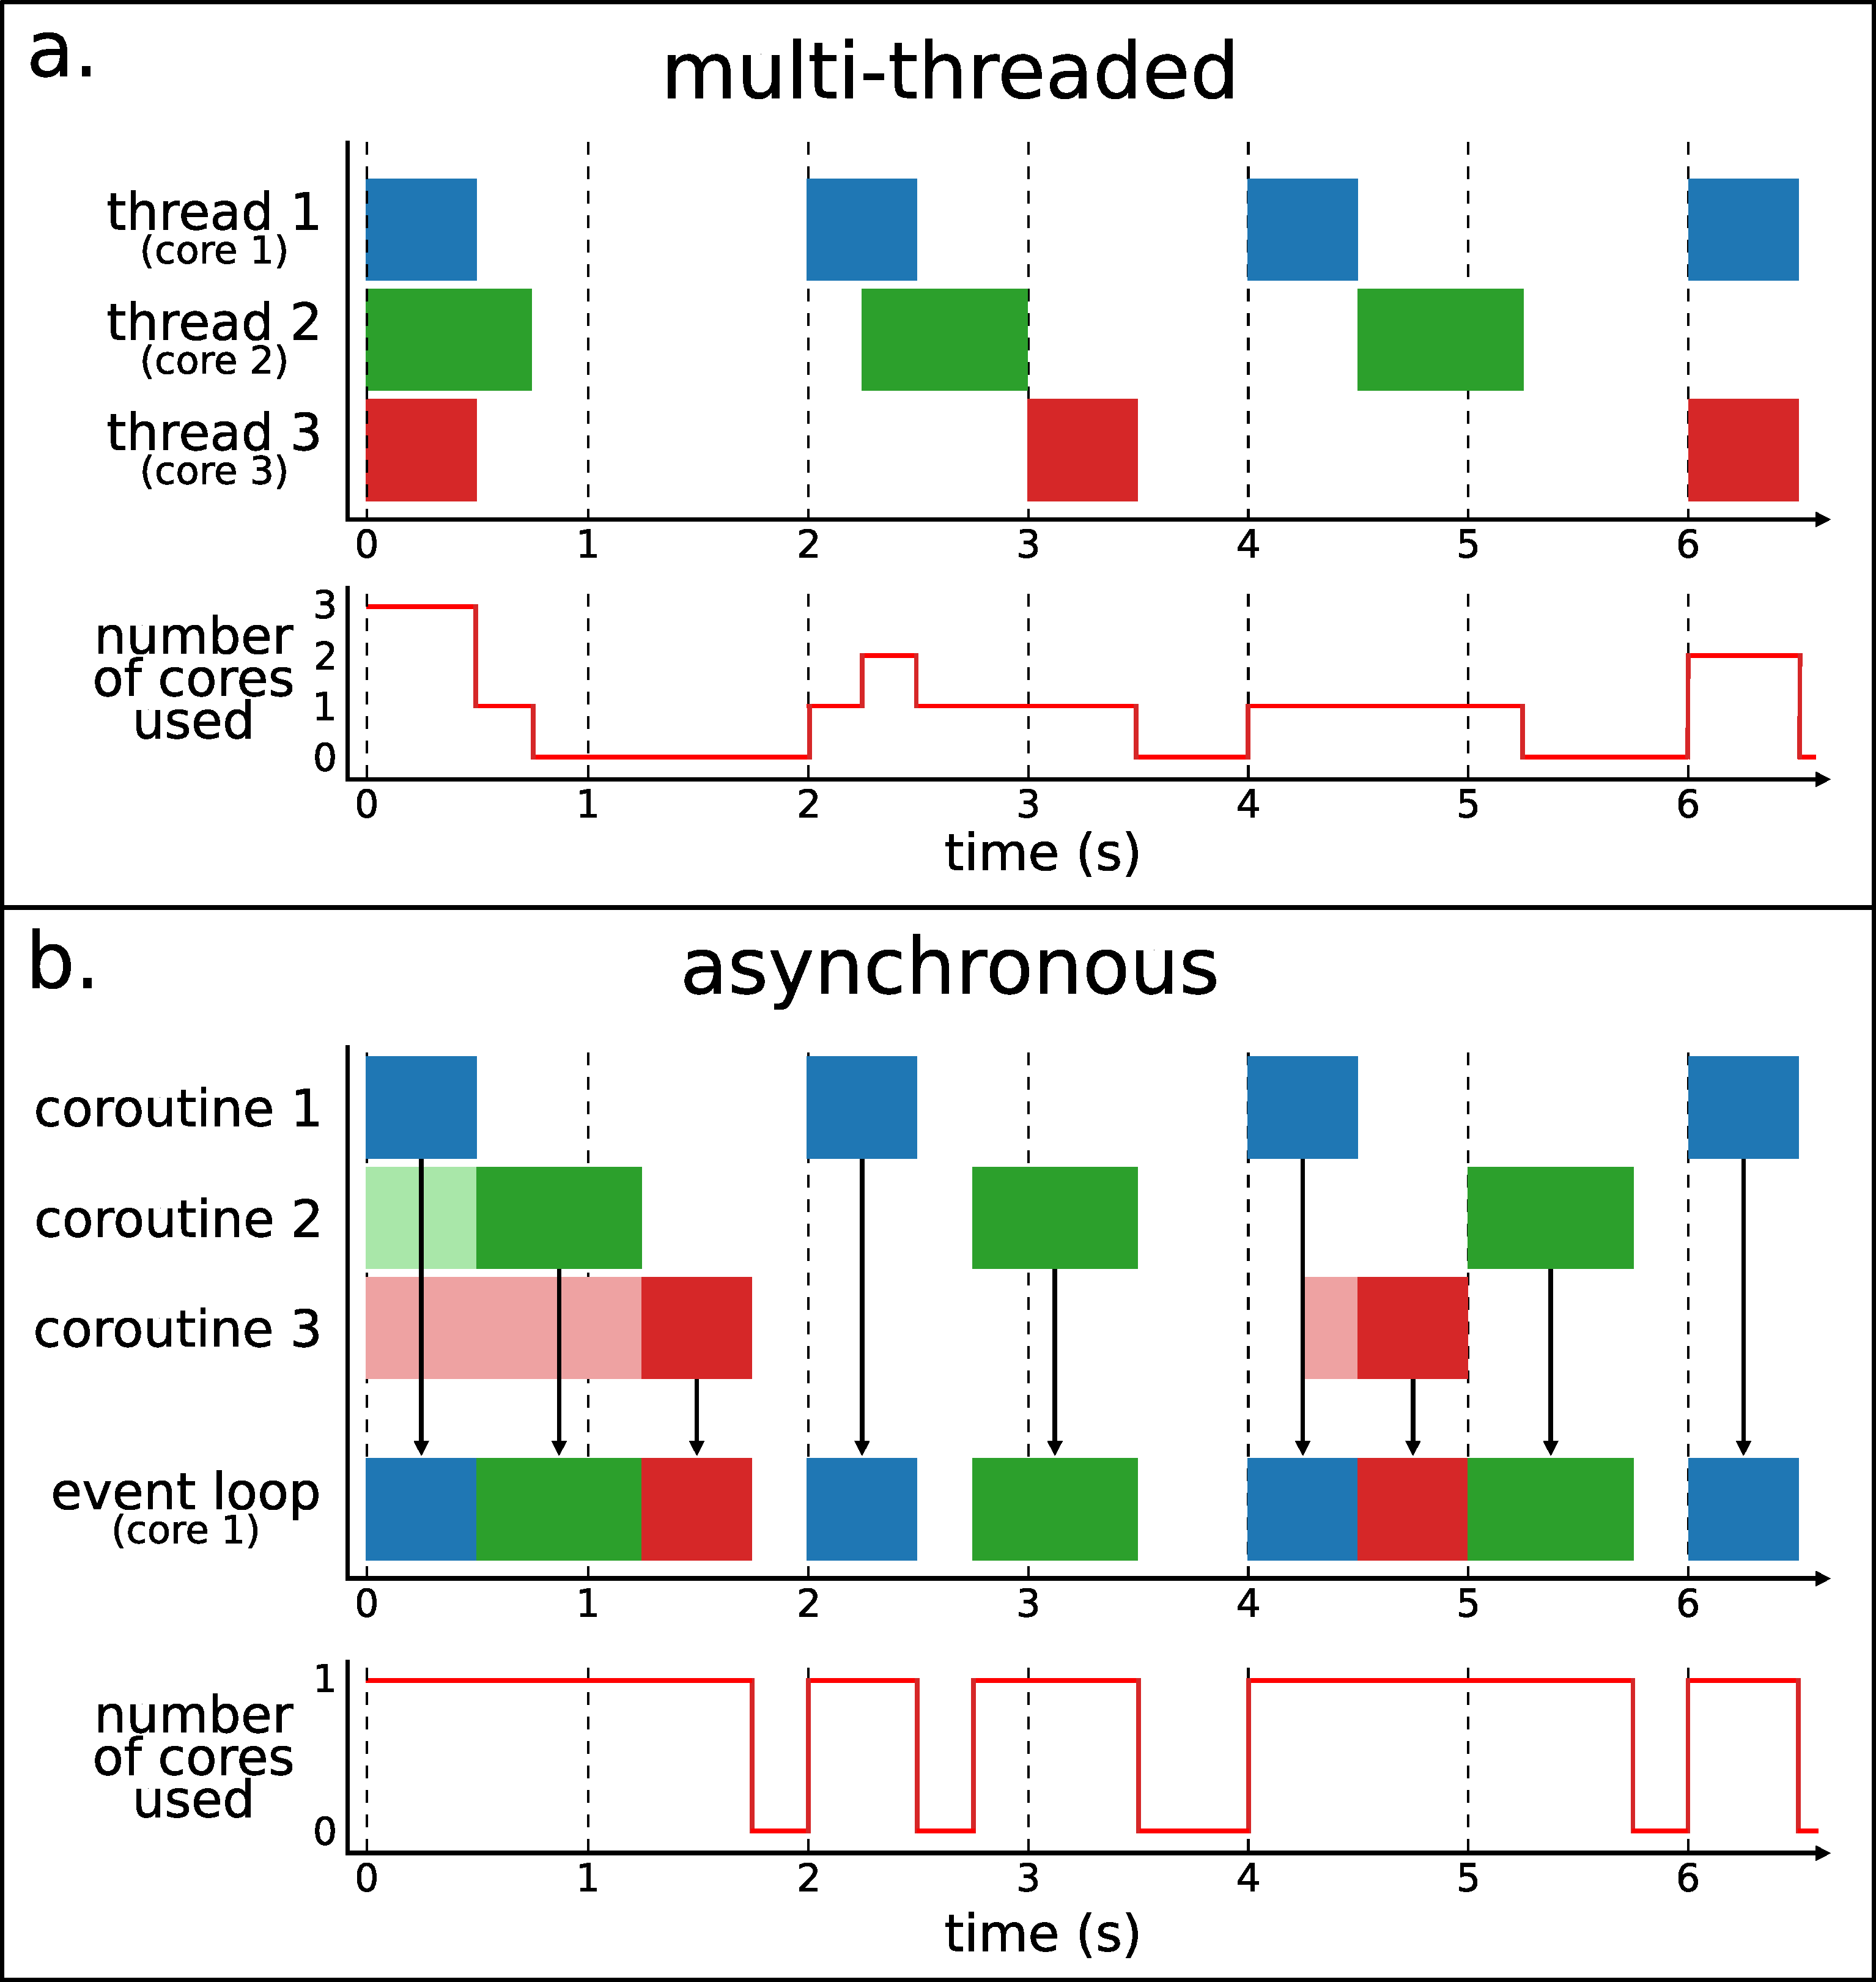
\includegraphics[width=0.9\linewidth]{images/async.pdf}
\end{center}
\caption[Multi-threaded vs asynchronous programming]{A comparison of multi-threaded vs asynchronous programming. This example uses a \textcolor{blue}{blue} task that takes \SI{0.5}{\second} to execute and then waits for \SI{1.5}{\second}, a \textcolor{ForestGreen}{green} task that takes \SI{0.75}{\second} and waits for \SI{1.5}{\second} and a \textcolor{red}{red} task that takes \SI{0.5}{\second} and waits for \SI{2.5}{\second}. These times are exaggerated for clarity, a typical pilot routine might take a second or less to run but then wait for anywhere between 10 and 60 seconds.
\\
\textbf{Top}: The three tasks with different execution periods (solid blocks) and wait times (blank) are run in a multi-threaded program. Each task is being run in an independent parallel thread on its own core, even though they rarely overlap and it is uncommon for multiple cores to be in use at the same time.
\\
\textbf{Bottom}: The same three tasks are run as coroutines in an asynchronous program. The event loop decides which coroutine to run on the single core, represented by the black arrows. This does lead to some coroutines being left waiting (lighter blocks) until the previous is finished, however the overall core usage is much more efficient.}
\label{fig:async}
\end{figure}

% ---------
\subsubsection{The check routines}

The coroutines within the pilot can be separated into two types: the check routines and the night marshal. Most of the coroutines are designed as monitors to regularly check different parts of the system, which fits well into the asynchronous model. These check routines are as follows:

\begin{itemize}

\item \texttt{check\_hardware} monitors the hardware daemons, checking every 60 seconds that they are all reporting their expected statuses. It does this using the hardware monitor functions, which are described later. If an abnormal status is returned then the pilot will pause (see below) and a series of pre-set recovery commands generated by the monitor are executed in turn. While in recovery mode the pilot will check the monitors more frequently. If the commands work and the status returns to normal the pilot is resumed, but if the commands are exhausted without the problem being fixed then an alert is issued that the system requires human intervention and the pilot triggers an emergency shutdown.

\item \texttt{check\_dome} is a backup to the primary hardware check routine. \texttt{check\_hardware} does monitor the dome along with the other hardware daemons, but \texttt{check\_dome} provides a simple, dedicated backup to ensure the dome is closed when it should be and to raise the alarm if it is not.

\item \texttt{check\_flags} is a routine that monitors the system flags, most notably those created by the conditions daemon (see Sec.~\ref{sec:conditions}). If any of the conditions flags are bad then the dome daemon will enter lockdown and close the dome on its own (see Sec.~\ref{sec:dome}), but the \texttt{check\_flags} routine will abort exposures, pause the pilot and ensure it is not resumed until the flag is cleared. When conditions are clear again the pilot will reopen the dome and allow normal operations to be restored. The \texttt{check\_flags} routine also monitors the system mode and will pause the pilot if it is set to manual mode or exit if set to engineering mode (see Section~\ref{sec:mode}).

\item \texttt{check\_scheduler} is a routine that queries the scheduler daemon every 10 seconds to find the best job to observe. If the pilot is currently observing the scheduler will either return the database ID of the current pointing, in which case the pilot will continue with the current job, or a new ID which will lead to the pilot interrupting the current job and moving to observe the new one. If the pilot is not currently observing (either it is the start of the night, resuming from being paused or the previous pointing has just completed) then it will begin observing whatever the scheduler returns. The details of how the scheduler decides which target to observe are given in Sec.~\ref{sec:scheduler}. The ID returned is then passed to the observe (OBS) task run by the night marshal.

\end{itemize}

% ---------
\subsubsection{The night marshal}

The above check routines are support tasks for the primary routine, which is called the \texttt{night\_marshal}. Unlike the check routines the night marshal does not contain a repeating loop, instead it runs through an ordered list of set tasks as the night progresses, based on the altitude of the Sun. Each key task is contained in a separate \proglang{Python} observation script, which contains the commands to send to the hardware daemons. Each is run spawning a new coroutine, meaning that while they are running the other routines such as the check tasks can continue. In the order they are performed during the night, the night marshal tasks are:

\begin{enumerate}

\item STARTUP, run immediately when the pilot starts. The night marshal executes the \texttt{startup} script which powers on the camera hardware, unparks the mount, homes the filter wheels and cools the CCDs down to their operating temperature of \SI{-20}{\celsius}.

\item DARKS, run after the system start up is complete before opening the dome. This executes the \texttt{takeBiasesAndDarks} script to take a set number of bias and dark frames at the start of the night, usually nine of each.

\item OPEN, run once the Sun reaches \SI{0}{\degree} altitude. It simply executes the \texttt{dome~open} command. If the pilot is paused due to bad weather or a hardware fault then the night marshal will wait and not open until the weather improves or fault is fixed. If it is never resolved then the night marshal will remain here until the end of the night and the shutdown timer runs out (see below).

\item FLATS, run once the dome is open and the Sun reaches \SI{-1}{\degree}. This executes the \texttt{takeFlats} script, which moves the telescope into anti-sun position and then takes flat fields in each filter, stepping in position between exposure and automatically increasing the exposure time as the sky darkens. See Section~\ref{sec:flats} for details of the flat field routine.

\item FOCUS, run once the Sun reaches \SI{-11}{\degree}. This executes the \texttt{autoFocus} script, which finds the best focus position for each of the unit telescopes. See Section~\ref{sec:autofocus} for details of the autofocus routine. If the routine fails for any reason the previous nights' focus positions are restored.

\item OBS (short for ``observing''), begun once the Sun reaches \SI{-15}{\degree} and continuing for the majority of the night until the Sun reaches \SI{-15}{\degree} again in the morning. When a database ID is received from the scheduler via the \texttt{check\_schedule} routine the \texttt{observe} script is executed. The script queries the observation database (see Sec.~\ref{sec:obsdb}) to get the coordinates and exposure settings for that pointing and then sends the commands to the mount and exposure queue daemons. Once a job is finished, either through completing all its exposures or being interrupted, the entry in the database status entry is updated and the routine awaits the next job from the scheduler.

\item FLATS is repeated once the Sun reaches \SI{-10}{\degree} in the morning, using the same script but this time increasing the exposure times as the sky brightens.

\end{enumerate}

These scripts are self-contained programs which mean they can also be called independently, for example if the pilot is not running and a manual observer wants to run the autofocus routine they can use the command \texttt{obs\_script~autoFocus}.

Once the night marshal has completed all of its tasks it exits. The pilot has an internal shutdown timer which set at the beginning of the night to when the rising Sun will reach \SI{0}{\degree} altitude again. When this time is reached the pilot then runs the \texttt{shutdown} script, which powers off the cameras, parks the mount and ensures the dome is closed. This is on a separate timer to the rest of the night marshal tasks, meaning if something goes wrong during the night the system will always shut down in the morning. It is also possible for the system to emergency shut down during the night, which will occur if a critical error occurs that can not be solved without human intervention (see the definition of a critical conditions flag in Sec.~\ref{sec:conditions}). This ends the pilot for the night, and it falls on whoever checks the alert to restart it if they decide the cause of the alert is resolved.

% ---------
\subsubsection{The hardware monitors}

WIP

\end{colsection}

% ~~~~~~~~~~~~~~~~~~~~

\subsection{Conditions monitoring}
\label{sec:conditions}
\begin{colsection}

The conditions daemon is a support daemon that runs on the central server. It takes in readings from the three local weather stations next to the GOTO dome on La Palma, as well as other sources such as internal sensors, every 10 seconds. The daemon processes these inputs into a series of output flags, which have a value of 0 (Good), 1 (Bad) or 2 (ERROR). If any of the flags are marked as not Good then the overall conditions are bad: the dome will close (Sec.~\ref{sec:dome}) and the pilot will pause (Sec.~\ref{sec:pilot}). The conditions daemon is run centrally on the main server because it deals with site-wide values, so when the second instrument is built it is envisioned that they will both share the same conditions daemon.

Each conditions flag has a limit below or above which the flag will turn from good to bad. For categories with multiple sources (for example each of the three weather stations gives an independent external temperature reading) then the limit will be applied to each and if any are found to be bad then the flag is set. Each category also has two parameters, the bad delay and the good delay. These are the time the conditions daemon waits between an input going bad/good and setting the flag accordingly, which has the effect of smoothing out any sudden spikes in a value and ensures the dome will not be opening and closing too often. Certain flags are also marked as critical flags, for conditions that will not be solved by the system pausing and will need human intervention to fix. Alerts are sent out in the form of automated messages to the system Slack channel, with further email and text messages being considered before the system moves to fully unsupervised operations. Alerts are only sent out when critical flags are set, which is why some flags have a normal and a more serious critical version.

An explanation of all the conditions flags is given below. Note the exact values of limits and delay times are often subject to adjustment as commissioning occurs in different weather conditions and seasons.

\begin{itemize}
\item \texttt{rain}: A very simple flag, it is set to bad immediately if any of the weather stations report rain, and will only be cleared after 10 minutes of no more rain reported. In practice rain usually coincides with high humidity, meaning the \texttt{rain} and \texttt{humidity} flags often overlap.

\item \texttt{humidity}: The critical humidity limit is 75\%, with a bad delay of two minutes and a good delay of five minutes.

\item \texttt{temperature} and \texttt{ice}: The \texttt{temperature} flag is set if the temperature drops below \SI{1}{\celsius} for two minutes, and has a good delay of five minutes. The \texttt{ice} flag uses the same input but is set if the temperature is below \SI{0}{\celsius} for one hour and will only clear if the temperature is above freezing for 24 hours. The \texttt{ice} flag is a critical flag, meaning it will prevent the system from opening until manually cleared (in this case the dome has been checked for any ice formation).

\item \texttt{windspeed}: Another simple flag that gets set if the windspeed is above 40 km/h, with the same two minute bad delay and five minutes good delay as the other external flags.

\item \texttt{internal}: A combination flag for the two internal temperature and humidity sensors within the dome. These have very extreme limits, a humidity of above 90\% or a temperature of below \SI{-3}{\celsius}, which should never be reached under normal circumstances due to the internal dehumidifier. This flag therefore is a backup for an emergency case, when either the dehumidifier is not working or the dome has somehow opened in bad conditions. This is a critical flag, in order to alert that something is wrong inside the dome.

\item \texttt{link}: The conditions daemon also monitors the external internet link to the site, by pinging the Warwick server and other public internet sites. If these pings are unsuccessful after a minute then the \texttt{link} flag gets set to bad. It is technically possible for the system to observe without any internet link, but it is an unnecessary risk as if anything went wrong alerts could not be sent out and external users would not be able to log in.

\item \texttt{diskspace}: The amount of free disk space on the image data drive is also monitored, with the system shutting down and sending out an alert if there is less than 5\% space available. This is a critical flag, as currently space needs to be cleared manually.

\item \texttt{ups} and \texttt{low\_battery}: The conditions daemon will set the \texttt{ups} flag if the observatory has lost power and the system UPSs are discharging. Brief power cuts do occur on La Palma, but rarely for more than a few minutes. The \texttt{low\_battery} flag is a critical flag that gets triggered if the UPSs ever reach less than 75\% battery remaining, which would be a sign of a more serious problem that is worth alerting and forcing a shutdown until it is cleared.

\item \texttt{hatch}: A critical flag to detect if the access hatch into the dome has been left open. This flag is unique in that is is only valid in robotic mode; when in manual mode it is assumed that the hatch being opened is a result of someone operating the telescope. However once the system is observing robotically the hatch being open is a critical problem, as there is no way to close it remotely and in the case of bad weather damage could be caused to the telescope.

\end{itemize}

\end{colsection}

% ~~~~~~~~~~~~~~~~~~~~

\subsection{The observation database}
\label{sec:obsdb}
\begin{colsection}

\begin{figure}[ht]
\begin{center}
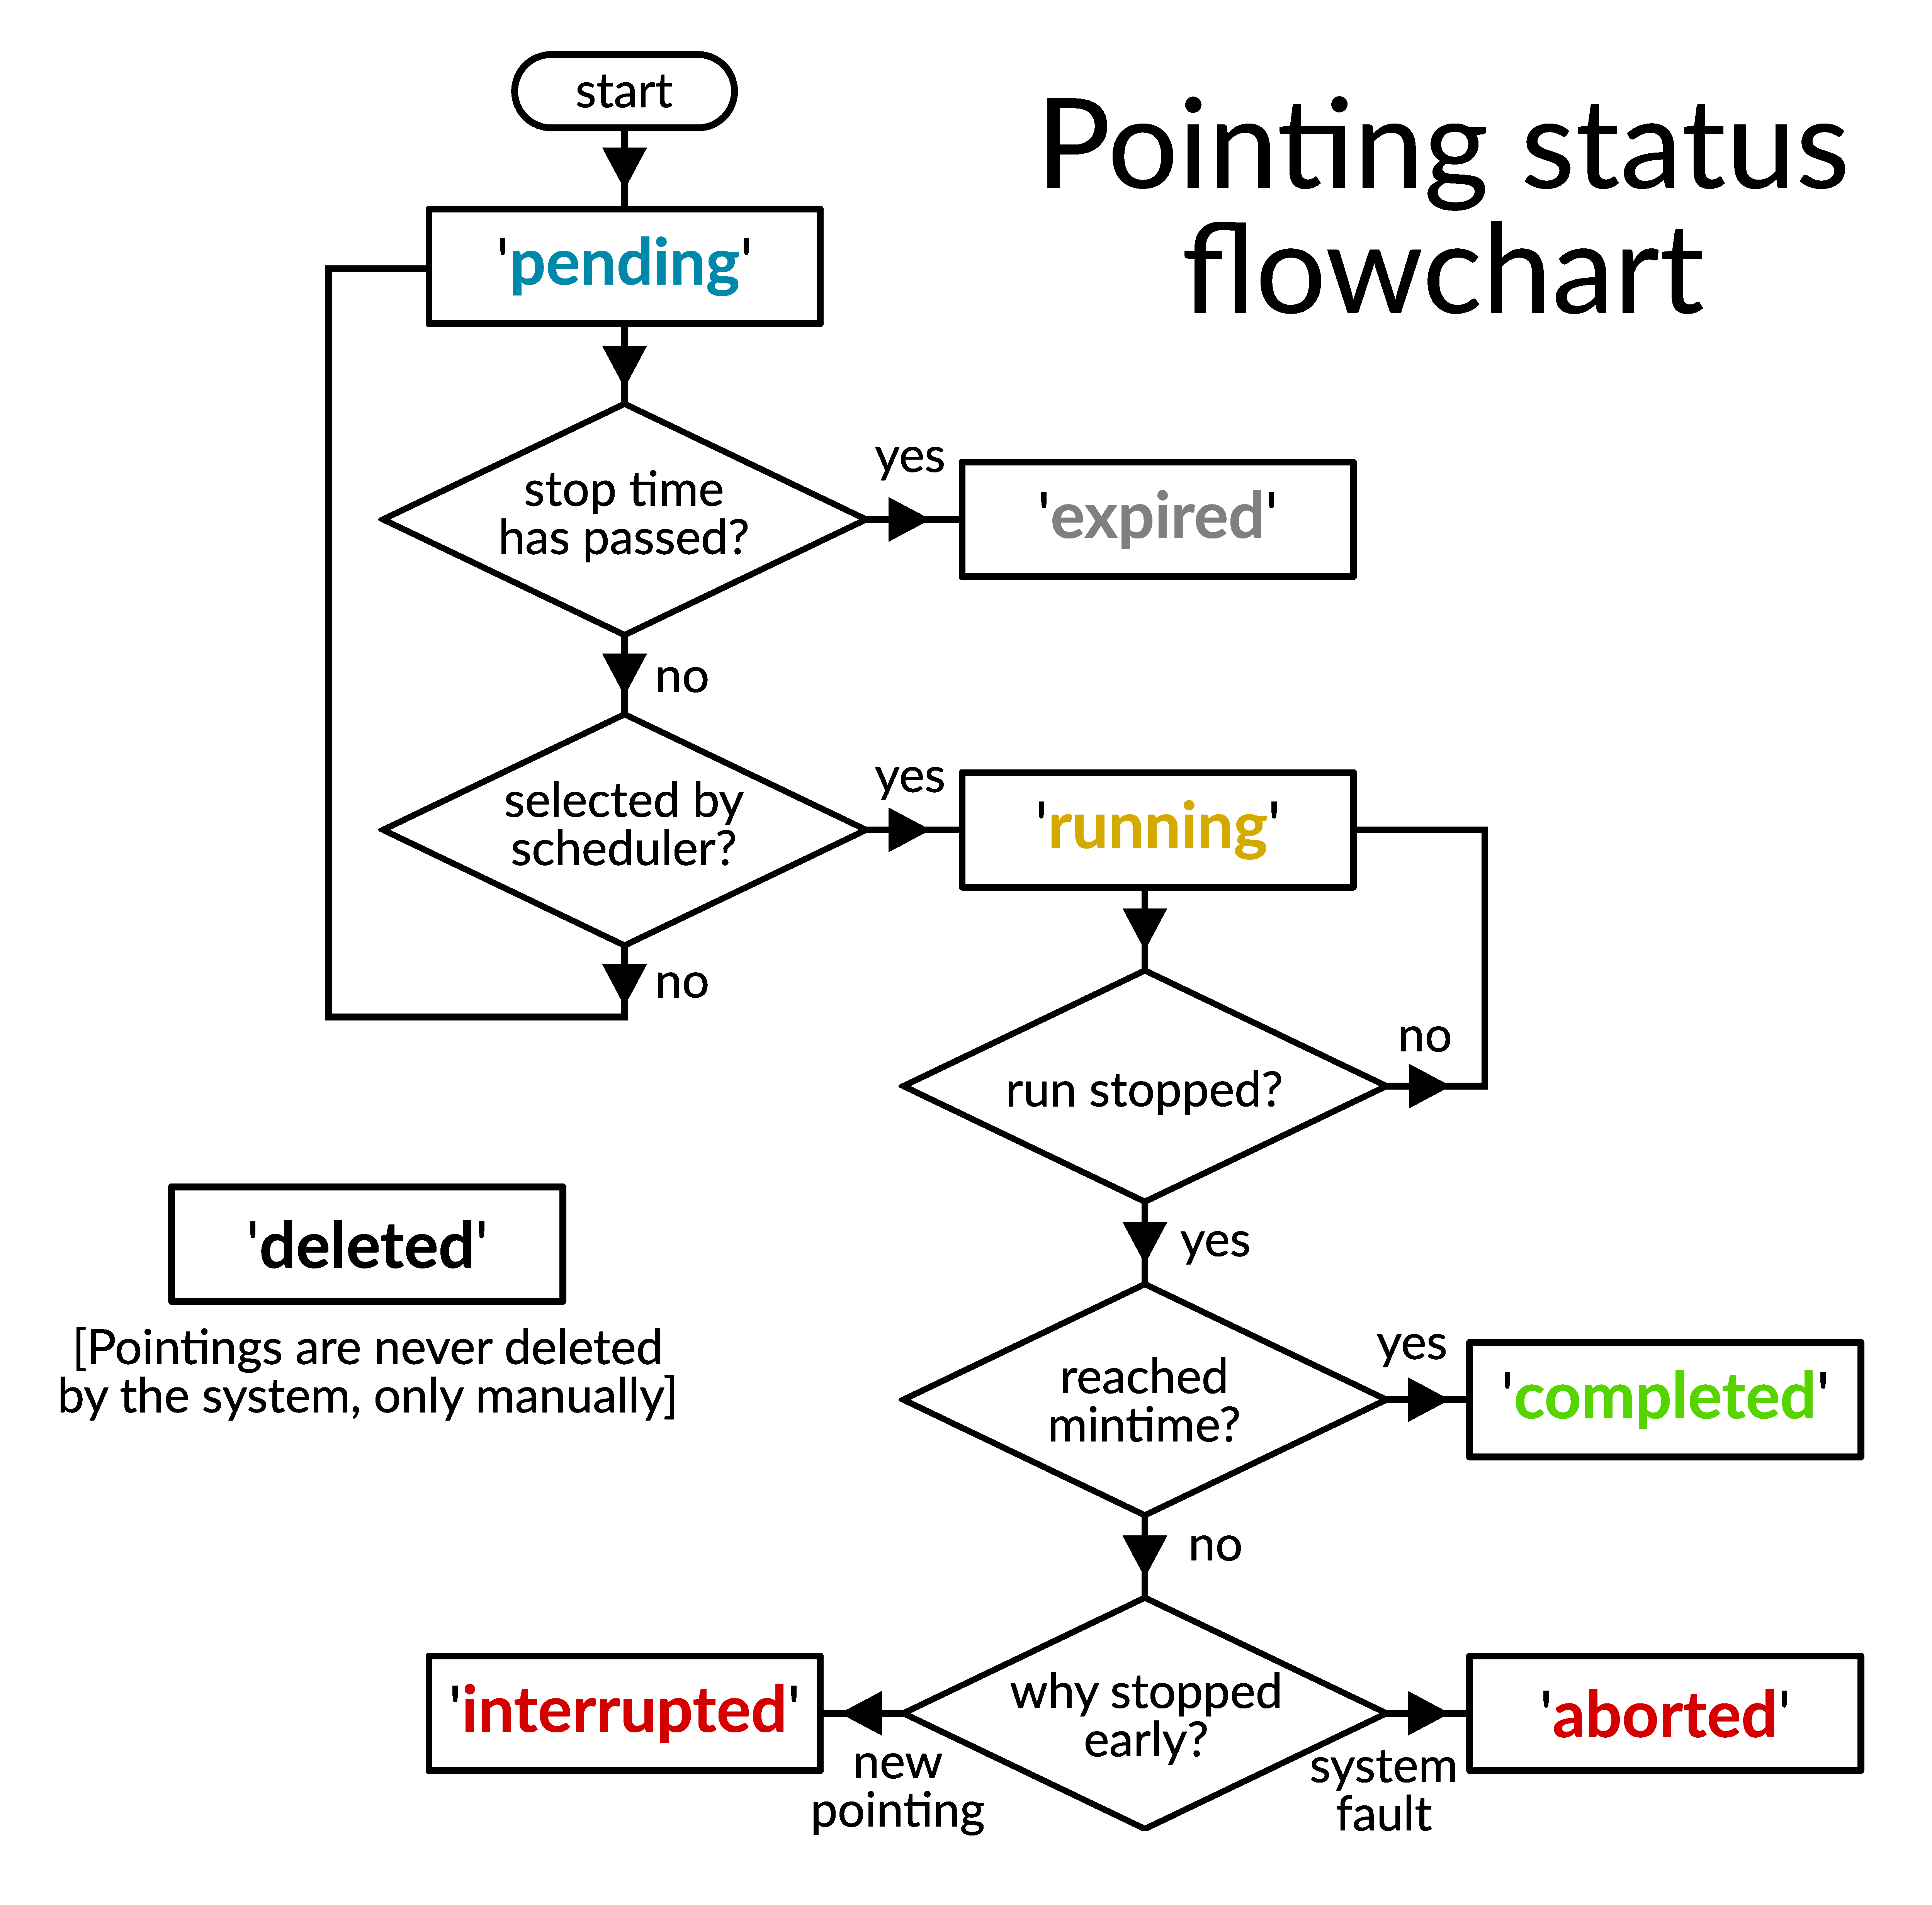
\includegraphics[width=9cm]{images/pointings.pdf}
\end{center}
\caption[Pointings]{A flowchart showing how the status of an entry in the pointings table can change.}
\label{fig:pointings}
\end{figure}

The scheduling system for \textsf{G-TeCS} is based around a MariaDB database, known as the observation database. The primary table in the database is for individual \textit{pointings}. These each represent a single visit of the telescope, with defined RA and Dec coordinates and a valid time range for it to be observed (a start time and a stop time) as well as other parameters.

Each pointing has a status value which is either \textit{pending}, \textit{running}, \textit{completed} or some other terminal status (\textit{aborted}, \textit{interrupted}, \textit{expired} or \textit{deleted}). Ideally a pointing passes through three stages: it is created as pending and sits around in the database, the scheduler eventually selects it and the pilot marks it as running, then if all is well when it is finished it is marked as completed. If it stays in the database and never gets observed it will eventually pass its defined stop time (if it has one) and will be marked from pending to expired by the database caretaker script. If the pointing is in the middle of being observed but is then cancelled before being completed it will be marked either interrupted (if the scheduler decided to observe another pointing of a higher priority) or aborted (in the case of a system problem such as having to close for bad weather). The deleted status is never set automatically, and is reserved for pointings being manually removed from the queue for whatever reason. A representation of the relationship between the pointing status values and how they progress is shown in Fig.~\ref{fig:pointings}.

As well as the target information (RA, Dec, target name) a pointing entry contain limits and constraints about when they can be observed. Each pointing can have a start and stop times set as already mentioned; the scheduler will only select pointings where the current time is within their valid range (and once the stop time has passed they will be marked as expired). Limits can also be set on minimum target altitude, minimum distance from the Moon, maximum Moon brightness (in terms of Bright/Grey/Dark time) and maximum Sun altitude. These constraints are applied by the scheduler to each pointing when deciding which to observe, and unless they all pass the pointing is deemed invalid. When created a pointing is also assigned a rank, usually from 0--9, as well as a True/False flag marking it as a time-critical Target of Opportunity (ToO). These are used when calculating the priority for the pointing, see Sec.~\ref{sec:scheduler}.

The commands to be executed once the telescope has slewed to a pointing are stored in the \textit{exposure\_sets} table. An exposure set defines what commands the pilot will give to the exposure queue daemon. The table has columns for the number of exposures to take, the exposure time and the filter to use. For example, a typical GOTO observation involves taking three 120 second exposures in the L filter followed by one each in the R, G and B filters. This would take up four entries in the pointings table, the first with number of exposures as 3 and filter as L and the rest with number of exposures as 1 and the individual filters. When the pointing is observed by the pilot it will add all linked sets to the exposure queue where each is executed in turn (See Sec.~\ref{sec:fli}).

Each entry in the pointings table can only be observed once. For observing a target more than once there also exists the \textit{mpointings} table, which contains information to dynamically re-generate pointings for a given target. An mpointing entry is defined with three key values: the requested number of observations, the time each should be valid in the queue and the time to wait between each observation. Each time the database caretaker script is run it looks for any entries in the mpointing table that still have observations to do and it creates another entry in the pointings table for that target. Setting the time values allows a lot of control over when pointings can be valid, for example scheduling follow-up observations a set number of hours or days after an initial pointing is observed.

\end{colsection}

% ~~~~~~~~~~~~~~~~~~~~

\subsection{Alert processing (the sentinel)}
\label{sec:sentinel}
\begin{colsection}

\begin{figure}[t]
\begin{center}
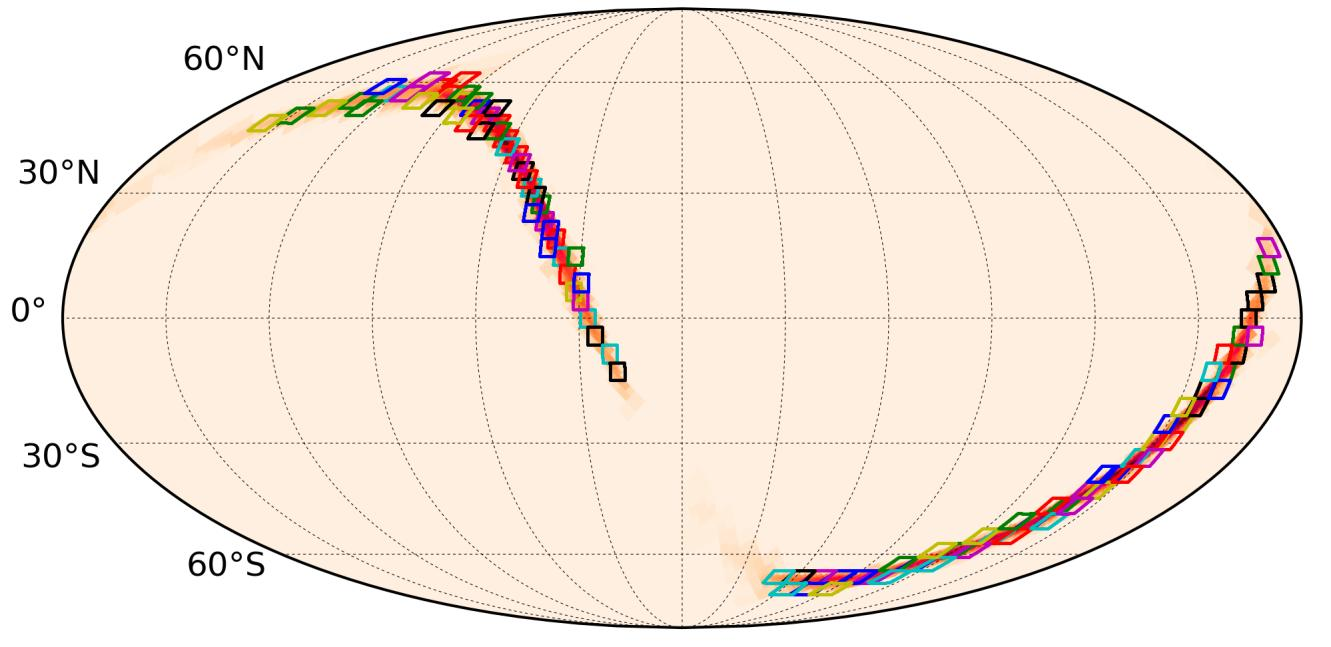
\includegraphics[width=14cm]{images/tiling.png}
\end{center}
\caption[The probability
 for GW151226]{The probability skymap for gravitational wave event GW151226~\citep{GW151226}, covered in tiles matching the field of view of GOTO in the four unit telescope configuration.}
\label{fig:tiling}
\end{figure}

In order for targets to be observed by GOTO in robotic mode they must have entries defined in the pointings (or mpointings) table in the observation database. These can be added manually, using a command line script or a web interface, but for automated observation they have to be inserted whenever an alert is detected. This is the job of the sentinel daemon, as shown in Fig.~\ref{fig:flow}. The sentinel acts as the alert listener for the system, taking any incoming targets and adding them to the database. For individual well-located sources like supernovae a single target is sufficient, but GOTO was designed to cover large areas resulting from gravitational wave skymaps. When an alert with a skymap is detected the sentinel calls functions from a Python module called \textsf{goto-tile}, which maps the skymap onto the fixed GOTO all-sky grid and returns a list of tile pointings and contained skymap probability within each. These are then added to the database by and processed by the scheduler daemon as described in Sec.~\ref{sec:scheduler}. An example of a skymap and the tiles output by \textsf{goto-tile} is shown in Fig.~\ref{fig:tiling}.

\end{colsection}

% ~~~~~~~~~~~~~~~~~~~~

\subsection{Scheduling observations}
\label{sec:scheduler}
\begin{colsection}

The scheduler daemon runs on the master server that also holds the primary observation database (see Sec.~\ref{sec:obsdb}). There is no specific command loop or hardware restrictions like in other daemons, but there are several advantages to having the scheduling calculations take place in their own daemon on the central server. Firstly, having the calculations done on the same machine as the database is more efficient when it comes to making queries, it is also a more powerful machine than the control computer that the pilot is running on. Furthermore when the second GOTO instrument is built having one scheduler that can speak to either pilot as required opens up further observation strategy opportunities.

The pilot queries the scheduler daemon every 10 seconds, and the job of the daemon is to return the database ID of the pointing that it has calculated is best to observe at the present time. This means GOTO operates under a ``just-in-time'' scheduling model, rather than creating a fixed plan at the beginning of the night of what to observe at each time. This system is very reactive to any incoming alerts as higher-priority pointings will immediately get included naturally in the calculation. The downside is that it less efficient for predefined targets than a night plan, which can be optimised before the night starts. However most of the time GOTO will normally be observing its all-sky survey, which has no strict timing requirements, and any other observations will be alerts entered by the sentinel daemon which could not be planned for.

When called, the scheduler will import the current queue of pointings from the observation database, filter out any that are invalid based on their individual constraints, then calculate a single priority value for each and find the pointing with the highest priority. The scheduling function then returns one of three results: carry on with the current observation, switch to a new observation or park the telescope in the case that there is no valid target. This decision will be returned to the pilot which will either continue what it is doing in the first case, or issue the necessary commands if required.

The first stage requires the scheduler to find the current queue by filtering the database pointings table. Firstly, pointings are selected based on their defined start and stop times by ensuring the current time is after their start time and before their stop time. Then the pointings are filtered in right ascension and declination by using the current local sidereal time to reject any pointings that would not be visible in the sky. After this initial basic filtering further constraints are applied by the scheduler based on the saved values for each pointing. Pointings have limits defined in Sec.~\ref{sec:obsdb} for physical constraints (altitude, Moon separation, Moon phase, Sun altitude) which are applied using the Constraints system in the \textsf{astroplan} Python module\cite{astroplan}. This ensures that only valid pointings are considered going forward.

The most important part of the scheduling function is calculating the priority value of each valid pointing in the queue. Each pointing entered into the GOTO database will have an assigned rank, which is fixed. The full priority is a floating point number that takes this rank and adds on values for other criteria so it can be easily compared to other pointings. The pointing with the smallest overall priority value is the highest priority to observe. The current criteria used are:

\begin{itemize}

\item The base rank of the pointing ($R$), which is fixed when created. Every pointing is given a rank between 0 and 9, and are deliberately biased towards prioritising gravitational wave events. Ranks 1 to 5 are reserved for these events, with ranks 6 to 9 reserved for other targets, which ensures that any incoming gravitational wave pointings will always be prioritised. Rank 0 is intended to never be used under normal circumstances, but it is a valid value that if set would outrank even gravitational wave events. Survey tiles all automatically have the lowest possible rank of 999, as they are the ever-present background and act as ``queue fillers'' in the system.

\item The repeat number ($N_{r}$), which accounts for the number of times that a particular target
or tile has already been observed, up to 99 times. This ensures that newer pointings are prioritised over later ones. Infinitely-repeating pointings like the survey tiles do not include this, which is why the survey tile ranks are static at 999.

\item The Target of Opportunity True/False flag ($F_{ToO}$). As pointings with the lowest priority value are preferred, pointings marked as ToOs will have $F_{ToO}=0$ and non-ToOs will have $F_{ToO}=1$.

\item The airmass of the pointing at the current time ($X$), calculated by the scheduler each time it is called. Including this will prioritise targets that are at lower airmasses and therefore provide the best quality data. Airmasses between 1 and 3 (altitudes between \SI{90}{\degree} and \SI{20}{\degree}) are converted into a value between 0 and 1.

\item For gravitational wave or other skymap pointings, the probability contained in the tile associated with the pointing ($P$). This will be calculated by the sentinel using \textsf{goto-tile} and linked to each pointing entered into the database (see Sec.~\ref{sec:sentinel}). The probability is inverted, as priority is ordered by the smallest value, therefore a tile with a 100\% probability of containing the source would have a value of $P=0$ and a tile with a 5\% probability would have $P=0.95$. Pointings that do not have probability values have the value set to 0 by default.

\item For survey tiles, the time since that tile was last observed ($T$). This is also scaled into a value in the range 0 to 1, where 0 corresponds to 7 days or more since the last observation.

\end{itemize}

These values are combined to form a single priority number using the formula:

\begin{equation}
Priority = 10 \times N_r + R + 0.1 \times F_{ToO} + 0.01 \times \left(\frac{a}{a+p+t}X + \frac{p}{a+p+t}P + \frac{t}{a+p+t}T\right),
\label{eq:priority}
\end{equation}

where $a$, $p$ and $t$ are weight factors for the airmass, probability and time-since-observed values. Each pointing in the queue has its priority calculated using Equation~(\ref{eq:priority}), the pointings are then sorted based on priority and the one with the smallest priority value is selected as the highest priority pointing.

\begin{sidewaystable}[b]
\caption{Some examples of calculated priority values. In this example the weight factors are $a=1$, $p=10$, and $t=10$. The final priority value is constructed using Equation~\ref{eq:priority}. The elements are coloured matching which part of the priority value they form --- the rank (\textcolor{red}{red}) and repeat number (\textcolor{orange}{orange}) form the integer part of the priority, the ToO flag (\textcolor{violet}{purple}) forms the first decimal place and the tie-break parameters (airmass, probability and time-since-observed, \textcolor{teal}{teal}) combined form the later decimal places.
}
\label{tab:priority}
\begin{center}
\begin{tabular}{clcclclclclcr}

\midrule
~&
\textbf{Target name} &
\textbf{$R$} &
\textbf{$N_r$} &
\textbf{ToO} &
$F_{ToO}$ &
\textbf{Am.} &
$X$ &
\textbf{Prob.} &
$P$ &
\textbf{Time} &
$T$ &
\textbf{Priority}
\\
\midrule

1 &
GW181202 T4 &
\textcolor{red}{1} &
\textcolor{orange}{0} &
True   & \textcolor{violet}{0}   &
1.1    & \textcolor{teal}{0.050} &
4.5\%  & \textcolor{teal}{0.955} &
$-$    & \textcolor{teal}{0}     &
\textcolor{orange}{~~}\textcolor{red}{1}.\textcolor{violet}{0}\textcolor{teal}{457} \\

2 &
GW181202 T9 &
\textcolor{red}{1} &
\textcolor{orange}{0} &
True   & \textcolor{violet}{0}   &
1.1    & \textcolor{teal}{0.050} &
0.3\%  & \textcolor{teal}{0.997} &
$-$    & \textcolor{teal}{0}     &
\textcolor{orange}{~~}\textcolor{red}{1}.\textcolor{violet}{0}\textcolor{teal}{477} \\

3 &
M31 &
\textcolor{red}{8} &
\textcolor{orange}{0} &
False  & \textcolor{violet}{1}   &
1.0    & \textcolor{teal}{0.000} &
$-$    & \textcolor{teal}{0}     &
$-$    & \textcolor{teal}{0}     &
\textcolor{orange}{~~}\textcolor{red}{8}.\textcolor{violet}{1}\textcolor{teal}{000} \\

4 &
GW181202 T3 &
\textcolor{red}{1} &
\textcolor{orange}{1} &
True   & \textcolor{violet}{0}   &
1.1    & \textcolor{teal}{0.050} &
9.1\%  & \textcolor{teal}{0.909} &
$-$    & \textcolor{teal}{0}     &
\textcolor{orange}{~1}\textcolor{red}{1}.\textcolor{violet}{0}\textcolor{teal}{435} \\

5 &
AT 2018bdk &
\textcolor{red}{6} &
\textcolor{orange}{2} &
True   & \textcolor{violet}{0}   &
1.0    & \textcolor{teal}{0.000} &
$-$    & \textcolor{teal}{0}     &
$-$    & \textcolor{teal}{0}     &
\textcolor{orange}{~2}\textcolor{red}{6}.\textcolor{violet}{0}\textcolor{teal}{000} \\

6 &
AT 2018bfe &
\textcolor{red}{6} &
\textcolor{orange}{2} &
True   & \textcolor{violet}{0}   &
1.2    & \textcolor{teal}{0.100} &
$-$    & \textcolor{teal}{0}     &
$-$    & \textcolor{teal}{0}     &
\textcolor{orange}{~2}\textcolor{red}{6}.\textcolor{violet}{0}\textcolor{teal}{005} \\

7 &
M101 &
\textcolor{red}{6} &
\textcolor{orange}{2} &
False  & \textcolor{violet}{1}   &
1.1    & \textcolor{teal}{0.050} &
$-$    & \textcolor{teal}{0}     &
$-$    & \textcolor{teal}{0}     &
\textcolor{orange}{~2}\textcolor{red}{6}.\textcolor{violet}{1}\textcolor{teal}{024} \\

8 &
Survey T31 &
\textcolor{red}{999} &
$-$ &
False  & \textcolor{violet}{1}   &
1.0    & \textcolor{teal}{0.000} &
$-$    & \textcolor{teal}{0}     &
4 days & \textcolor{teal}{0.429} &
\textcolor{orange}{}\textcolor{red}{999}.\textcolor{violet}{1}\textcolor{teal}{204} \\

9 &
Survey T33 &
\textcolor{red}{999} &
$-$                   &
False  & \textcolor{violet}{1}   &
1.0    & \textcolor{teal}{0.000} &
$-$    & \textcolor{teal}{0}     &
2 days & \textcolor{teal}{0.714} &
\textcolor{orange}{}\textcolor{red}{999}.\textcolor{violet}{1}\textcolor{teal}{340} \\

\midrule
\end{tabular}
\end{center}
\end{sidewaystable}

Some examples of calculated priority values using this method are given in Table~\ref{tab:priority}. The first two pointings are both gravitational wave tiles from the same (fictional) event. They have been inserted at rank 1, neither have been observed yet (meaning $N_r=0$), both are flagged as ToOs and both are at the same airmass. Therefore tie-breaking between the two comes down to the contained probability, and the tile with the higher contained probability (T4) is sorted first. There is another tile from the same event in the queue (T3) with an even higher contained probability, but as it has been marked as already having been observed once ($N_r=1$) is sorted further down below a pointing of M31 manually inserted at rank 8. Next there are three pointings all with the same rank ($R=6$) that have all been observed twice already ($N_r=2$). The first two transient events are both marked as ToOs while the pointing of M101 is not, so it is sorted last of the three. Choosing between the two transient targets comes down to the airmass, with the one currently higher in the sky (so at lower airmass) being sorted first. Finally two tiles from the all-sky survey are shown. These are both automatically fixed at rank 999, and in this case as they are both at the same airmass. Tile 31 is shown as being last observed 4 days ago while Tile 33 was observed only 2 days ago, so Tile 31 comes out with the higher priority.

As demonstrated in this example, priorities can be sorted easily in the first case by considering their repeat numbers, ranks and ToO flags. In the cases these are the same then the tiebreaking value is needed. This is most important when a new gravitational wave event comes in, which can result in up to one hundred new pointings being inserted at once at the same rank. The tiebreaker is a weighted combination of the airmass, contained probability (for skymap tiles) and time since last observation (for survey tiles). The exact weighting is shown in Equation~(\ref{eq:priority}) and depends on the values of $a$, $p$ and $t$. For standard non-skymap, non-survey pointings only airmass is considered, as $P$ is always set to 1 and $T$ is always 0 (as shown in Table~\ref{tab:priority}). Therefore pointings will be selected based on their altitude. For gravitational wave pointings the weighting between airmass and probability determines the observation strategy. Weighting airmass higher will prioritise pointings at a higher altitude and therefore increase typical data quality, but potentially at the loss of GW skymap coverage. On the other hand prioritising only probability would ensure the maximum possible coverage of the skymap, but low-altitude pointings might be selected when it might instead be better to wait until they were at a higher airmass. To attempt to find optimal weighting values many simulations were run with different skymaps and values. These simulations ran through a full night of observing, with the gravitational wave tiles inserted at a random time that day --- so simulating both an alert occurring during the night interrupting observations and the alert occurring during daytime so the pointings are there as soon as the system starts observing. Telescope downtime due to weather was also simulated as a Gaussian process with a 10\% chance of occurring and a typical timescale of 1 hour. The initial results of these simulations indicated a weighting of $a=1$ and $p=10$ provided the best optimisation between coverage and average airmass.

Once every pointing in the queue has had its priority calculated, the pointing with the smallest value is selected as the highest priority to observe. However before returning this pointing's database ID the  scheduler takes into account what the pilot is currently observing. In most cases the pilot will currently be observing a pointing previously given by the scheduler, and on the next check the scheduler will return that the same pointing is still the highest priority --- in which case pilot will continue observing. Even if the scheduler finds that a different pointing now has a higher priority it will not tell the pilot to change targets in the middle of observing unless the new pointing has the ToO flag set. Otherwise the pilot will wait until it has finished the current job. Finally if the scheduler finds nothing to do the pilot will park the telescope and wait for the next valid target.

\end{colsection}

% ~~~~~~~~~~~~~~~~~~~~

\end{colsection}

% ########################################
